\styledchapter[Proof of concept]{oplossing}
Om de PoC daadwerkelijk te maken moet er eerst gedefinieerd worden wat de scope is en hoe de PoC eruit gaat zien. De scope brengt in beeld wat er gedaan moet worden en wat de \acrfull{mvp} is. Op de \acrshort{mvp} kan de mock up gebaseerd worden. In dit hoofdstuk wordt de scope bepaald, delen van de mock up doorgelopen, uitleg gegeven over de PoC en kwaliteit van de code. Het hoofdstuk wordt afgesloten met een conclusie en advies

\section{User requirements verzamelen}\label{sec:ch7-user-requirements-verzamelen}
Om te begrijpen wat er gebouwd moet worden kunnen de behoeftes opgeschreven worden in de vorm van user stories. Een user story is de behoefte opgeschreven in een specifieke formaat om belangrijke informatie te achterhalen \cite{agile-user-story-template}. Een bekende formaat is de \textit{Connextra template} van Mike Cohn \cite{agile-user-story-template}: "\textbf{As a [role], I can [capability], so that [receive benefit]}". De template zorgt ervoor dat de rol (role), functie (capability) en reden (benefit) bekend is. In \autoref{fig:ch7-requirements} zijn alle user stories opgesteld, gegroepeerd in Epics. Bij elke user story is ook aangegeven of het \acrshort{mvp} is, welk prioriteit het heeft en de t-shirt size. De t-shirt size is een manier om op een hoog niveau aan te geven hoeveel werk een user story vereist. Een \textbf{S} vereist weinig werk terwijl \textbf{XL} veel werk vereist.

\begin{figure}[hbt!]
  \centering
  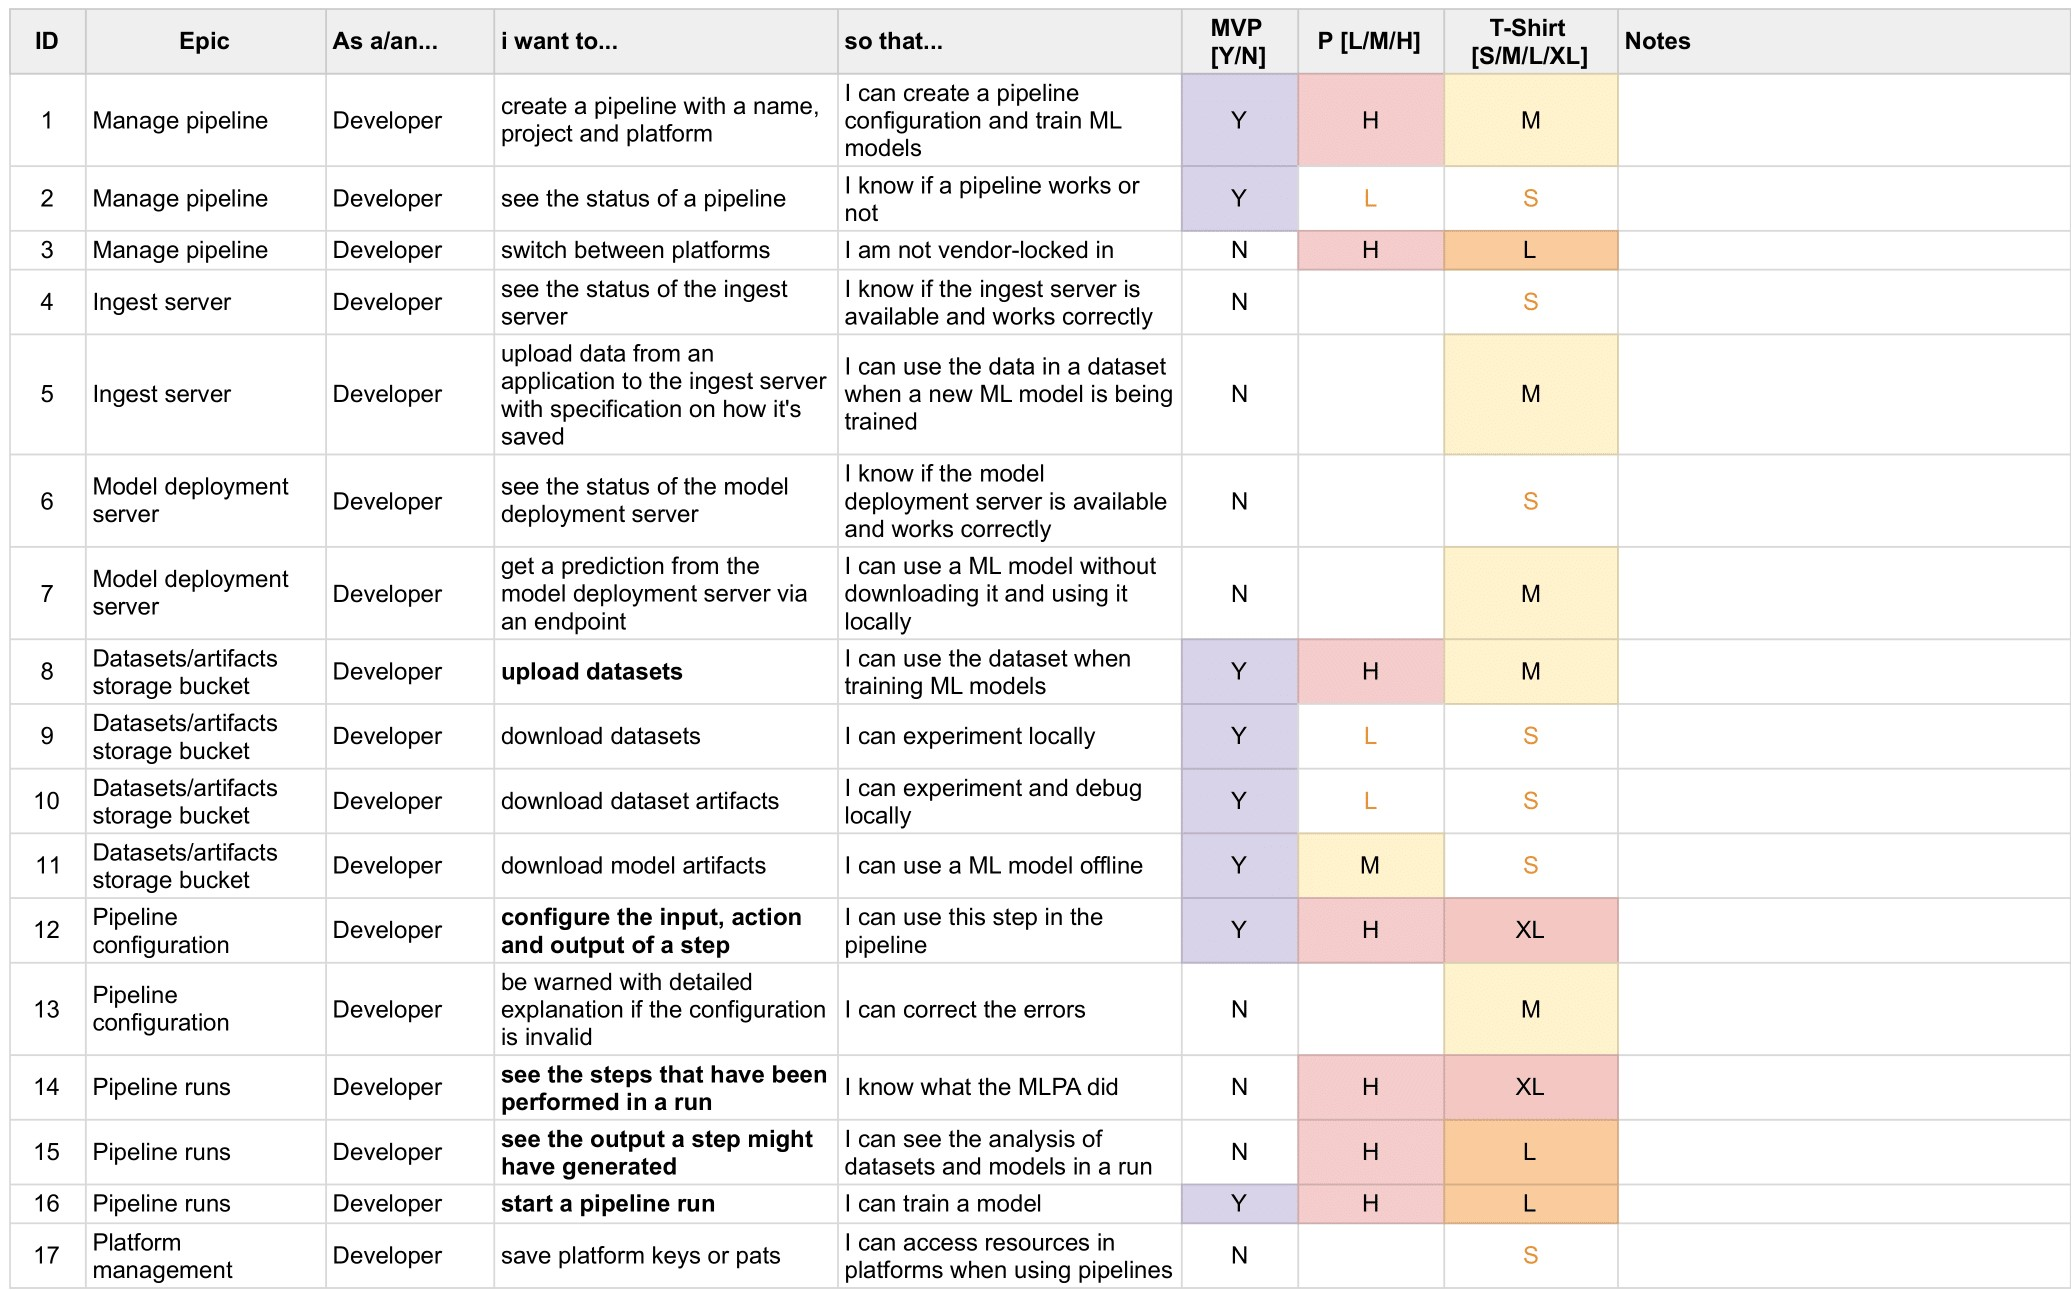
\includegraphics[width=1\textwidth]{chapter-7/requirements.jpg}
  \caption{Requirements opgesteld voor de proof of concept.}
  \label{fig:ch7-requirements}
\end{figure}

De user stories zijn opgesteld in samenwerking met de begeleiders van NGTI over het hele afstudeerproces. Nu de requirements zijn opgesteld, kan een Kanban bord opgericht worden om sprints te maken.

\newpage

\subsection{Requirements vertalen naar een scrum bord}\label{subsec:ch7-requirements-vertalen-naar-een-scrum-bord}
Een Kanban bord is een werkwijze om visueel aan te geven in welke stadia een taak is in het proces \cite{atlassian-kanban-board}. Taken in een Kanban bord vallen altijd onder een kolom om de status aan te geven. Een kolom kan bijvoorbeeld "todo", "doing", of "done"\space zijn. Een scrum bord is een vorm van een Kanban bord waarbij taken in een sprint zijn ingepland \cite{forecast-scrum-board}. Een sprint is een vaste periode van bijvoorbeeld een of twee weken waarin gewerkt wordt aan de ingeplande taken. Dit verschilt met een Kanban bord waarbij taken op elk moment toegevoegd kunnen worden. In software development kan dit niet; sprints zorgen ervoor dat er geen \gls{scope-creep} plaats vindt.

De user stories uit \autoref{fig:ch7-requirements} zijn vertaalt naar tickets in het scrum bord. Een user story is opgesplitst in meerdere tickets. Dit is het geval met bijvoorbeeld user story "upload datasets" (ID 8). Om deze functionaliteit te bouwen moet een storage bucket beschikbaar zijn en in de frontend de mogelijkheid zijn om dit te doen. In \autoref{fig:ch7-trello-w1-start} zijn de tickets aangemaakt met relevante labels om aan te geven bij welke epic een ticket hoort, of het \acrshort{mvp} is, de prioriteit en t-shirt size.

\begin{figure}[hbt!]
  \centering
  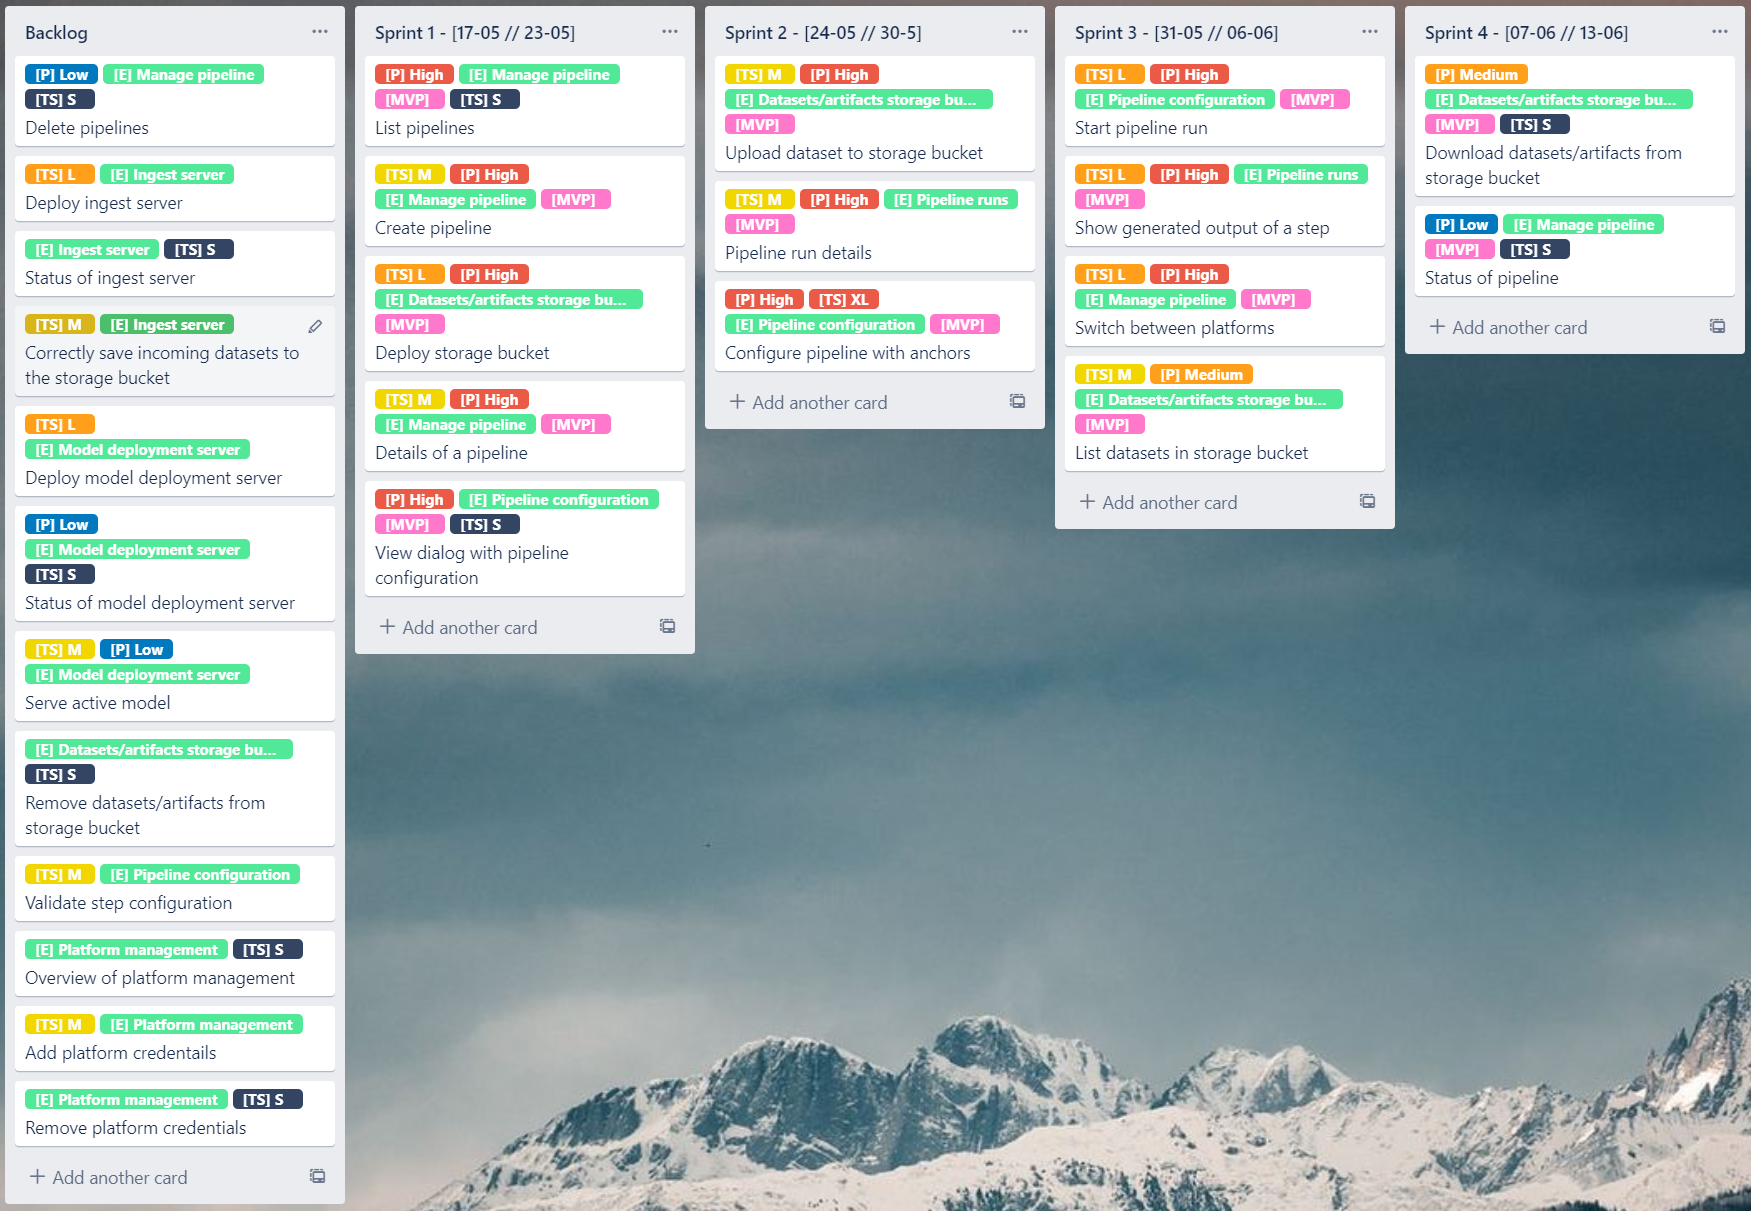
\includegraphics[width=0.99\textwidth]{chapter-7/trello-w1-start.png}
  \caption{Sprint 1.}
  \label{fig:ch7-trello-w1-start}
\end{figure}

In het ontwikkelproces is na elke sprint het scrum bord opnieuw bekeken om te reflecteren op de afgelopen sprint en de komende sprints opnieuw in te plannen als dit nodig was. Nu de tickets aangemaakt zijn en de \acrshort{mvp} is vastgesteld, kan de mock up gemaakt worden.

\section{Mock up van de proof of concept}\label{sec:ch7-mock-up-van-de-proof-of-concept}
De mock up is bedoeld om te laten zien hoe de frontend van de PoC eruit gaat zien. Dit geeft ook de kans om te controleren of de \acrfull{ui} logisch in elkaar zit. Om de mock up te ontwerpen is gebruik gemaakt van Adobe XD \cite{adobe-xd}. De mock up bevat alleen functionaliteiten die \acrshort{mvp} zijn. 

Een pipeline wordt aangemaakt door het invullen van de naam en project (bijlage \ref{appendix:mockup-overview-and-create-pipeline}). Na het aanmaken van een pipeline kan erop geklikt worden. In \autoref{fig:ch7-mockup-mvp-pipeline-details} is de mock up van de details van een pipeline te zien. Op deze pagina is de status van de pipeline, configuration, dataset/\glspl{artifact} en runs te zien.

\begin{figure}[hbt!]
  \centering
  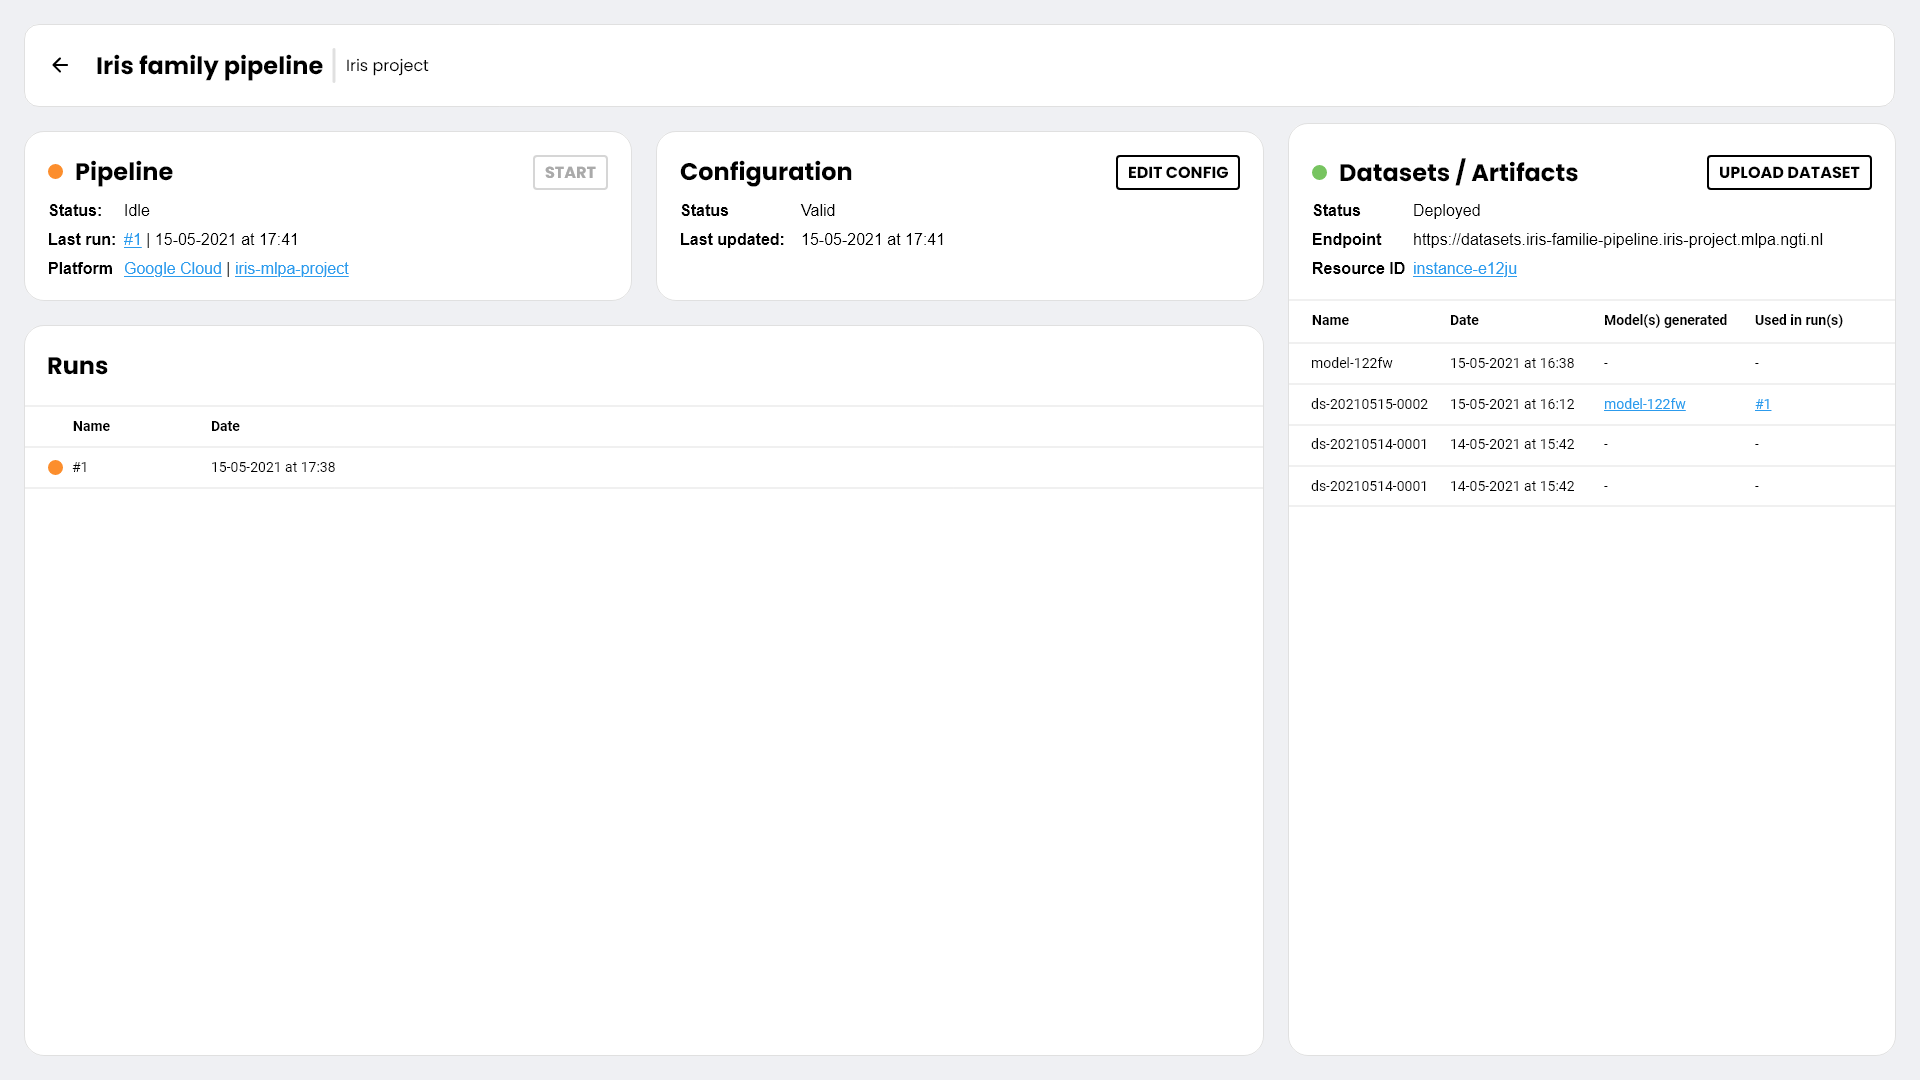
\includegraphics[width=0.99\textwidth]{chapter-7/[mvp]-pipeline-details.png}
  \caption{Mock up van de pipeline details pagina.}
  \label{fig:ch7-mockup-mvp-pipeline-details}
\end{figure}

De configuration is een Python script dat door de developer is gedefinieerd. De script wordt uitgevoerd als de pipeline wordt gestart en bevat de stappen uit \autoref{fig:ch4-model-lifecycle-oreilly}. Stappen zoals "Model deployment" en "Model feedback" vallen uit de scope. In de datasets/\glspl{artifact} sectie kan de developer datasets en artefacts up- en downloaden. Als laatste kan de developer de status van de pipeline en run zien. Een run is een individuele run als een pipeline wordt gestart. Mock ups van andere gedeeltes van de PoC is te vinden in bijlage \ref{appendix:mockup-configuration-dialog}. Nu het voorwerk is gedaan, kan code voor de PoC geschreven worden.

\section{Wijzigingen in het architecturaal ontwerp}\label{sec:ch7-wijzigingen-in-het-architecturaal-ontwerp}
Tijdens het ontwikkelproces is naar voren gekomen dat het orkestreren van infrastructuur in een cloud platform met een tool niet de juiste werkwijze is. Een orkestratietool werkt zoals uitgelegd in \autoref{subsec:ch5-wat-is-infrastructure-as-code} met een plan. De tool controleert de infrastructuur in een cloud platform aan de hand van het plan en past zo nodig de infrastructuur aan.

Gedurende het experiment kwamen geen problemen naar boven; echter bij het implementeren van een feature vertoonde Pulumi gedrag dat niet verwacht was. In \autoref{fig:ch7-reason-orchestration-tool-doesnt-fit} is een illustratie te zien ter ondersteuning van de uitleg. In de éérste stap (1) wordt middels code een plan beschreven waarbij een storage bucket aangemaakt moet worden. Pulumi valideert het plan en maakt vervolgens de storage bucket aan. Pulumi houdt intern bij met een manifest (M1) wat is aangemaakt, in dit geval een storage bucket. Bij de tweede stap (2) wordt Dataset A geüpload in de storage bucket. Pulumi houdt weer bij wat er aangemaakt is in de storage bucket met het manifest (M2). Bij de derde stap staat in het plan dat alleen Dataset B geüpload moet worden. Pulumi vergelijkt het plan met de manifest (M2) en ziet dat Dataset A niet in het plan staat. Pulumi verwijderd vervolgens Dataset A en upload Dataset B.

\begin{figure}[hbt!]
  \centering
  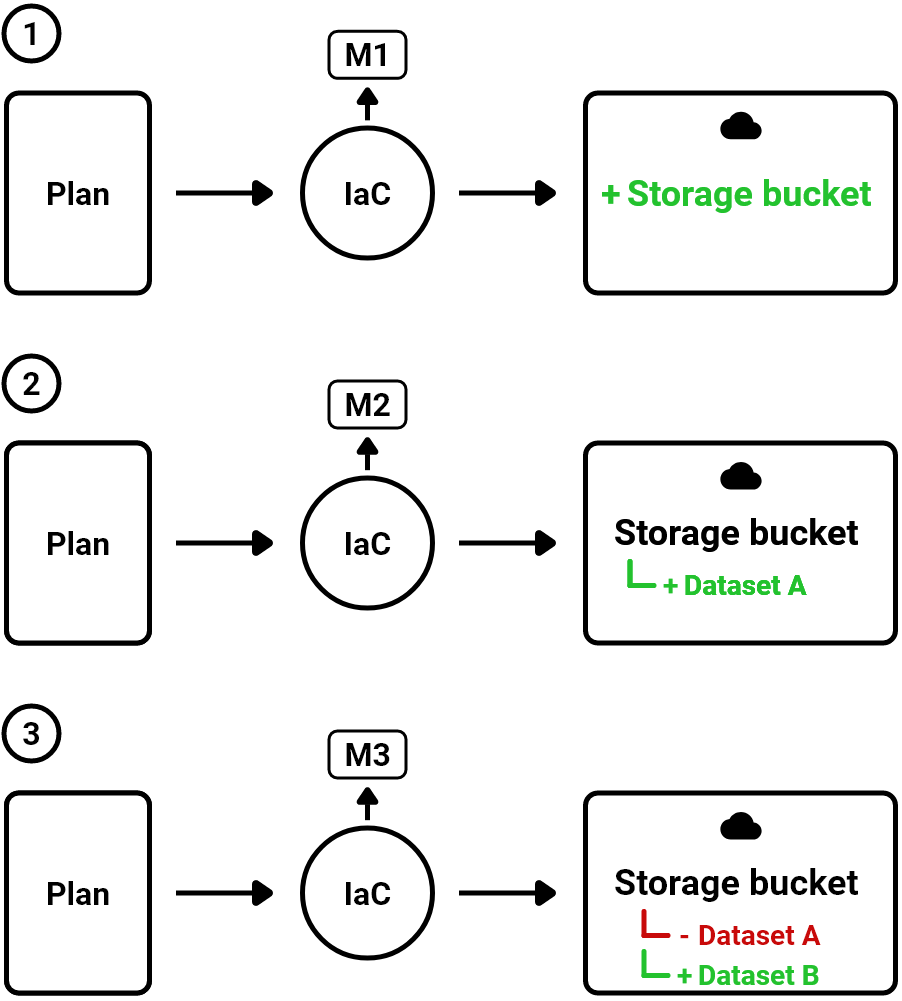
\includegraphics[width=0.6\textwidth]{chapter-7/reason-orchestration-tool-doesnt-fit.png}
  \caption{Gedrag van Pulumi met een incorrect plan.}
  \label{fig:ch7-reason-orchestration-tool-doesnt-fit}
\end{figure}

Pulumi verwacht dat de volledige infrastructuur in het plan beschrijft. Het is niet mogelijk om incrementeel de infrastructuur aan te passen. Voor de PoC is gekozen om verder te werken met libraries van de cloud platformen AWS, Google Cloud en Azure zelf. Na het onderzoeken of het mogelijk is om infrastructuur in te richten en naar de kwaliteit van de documentatie is gekozen om te werken met de libraries van Google Cloud en Azure. De documentatie van AWS is onoverzichtelijker en Amazon gebruikt unieke termen voor hun resources en services wat \cite{aws-sdk-javascript-docs}.

\section{De proof of concept}\label{sec:ch7-de-proof-of-concept}
In \autoref{sec:ch6-architecturaal-ontwerp} is kort uitgelegd dat de backend gebouwd wordt met Node.js en Express en de frontend met React.js en TypeScript. Voor de PoC is een GitHub repository aangemaakt waarin de front- en backend geïnitialiseerd is met behulp van de documentatie van de frameworks. In de volgende koppen wordt in een logische volgorde door de applicatie gelopen waarbij uitleg over de werking wordt gegeven met screenshots van de \acrshort{ui} en code als ondersteuning.

\subsection{Aanmaken van pipelines}\label{subsec:ch7-aanmaken-van-pipelines}
Om te beginnen moet een pipeline aangemaakt kunnen worden. In de frontend gaat dit met een dialoog (\autoref{fig:ch7-create-pipeline-dialog}). Hierin kan de naam, project en cloud platform aangegeven worden.

\begin{figure}[hbt!]
  \centering
  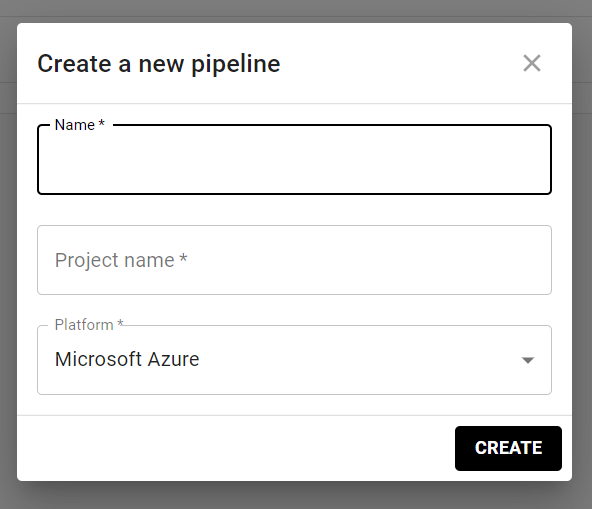
\includegraphics[width=0.5\textwidth]{chapter-7/poc-create-pipeline-dialog.png}
  \caption{Aanmaak dialoog van een pipeline.}
  \label{fig:ch7-create-pipeline-dialog}
\end{figure}

Zodra de developer klikt op de \textbf{Create} knop, wordt een request verstuurt van de frontend naar de backend. De backend stuurt de request naar een service dat ervoor zorgt dat de juiste acties uitgevoerd wordt. De service in \autoref{fig:ch7-create-pipeline-service} controleert welk platform er gespecificeerd is en spreekt de relevante functie aan. Als het platform bijvoorbeeld Google Cloud is, wordt de functie \(gc\_createBucket()\) op lijn 6 aangeroepen.

\newpage

\begin{figure}[hbt!]
  \centering
  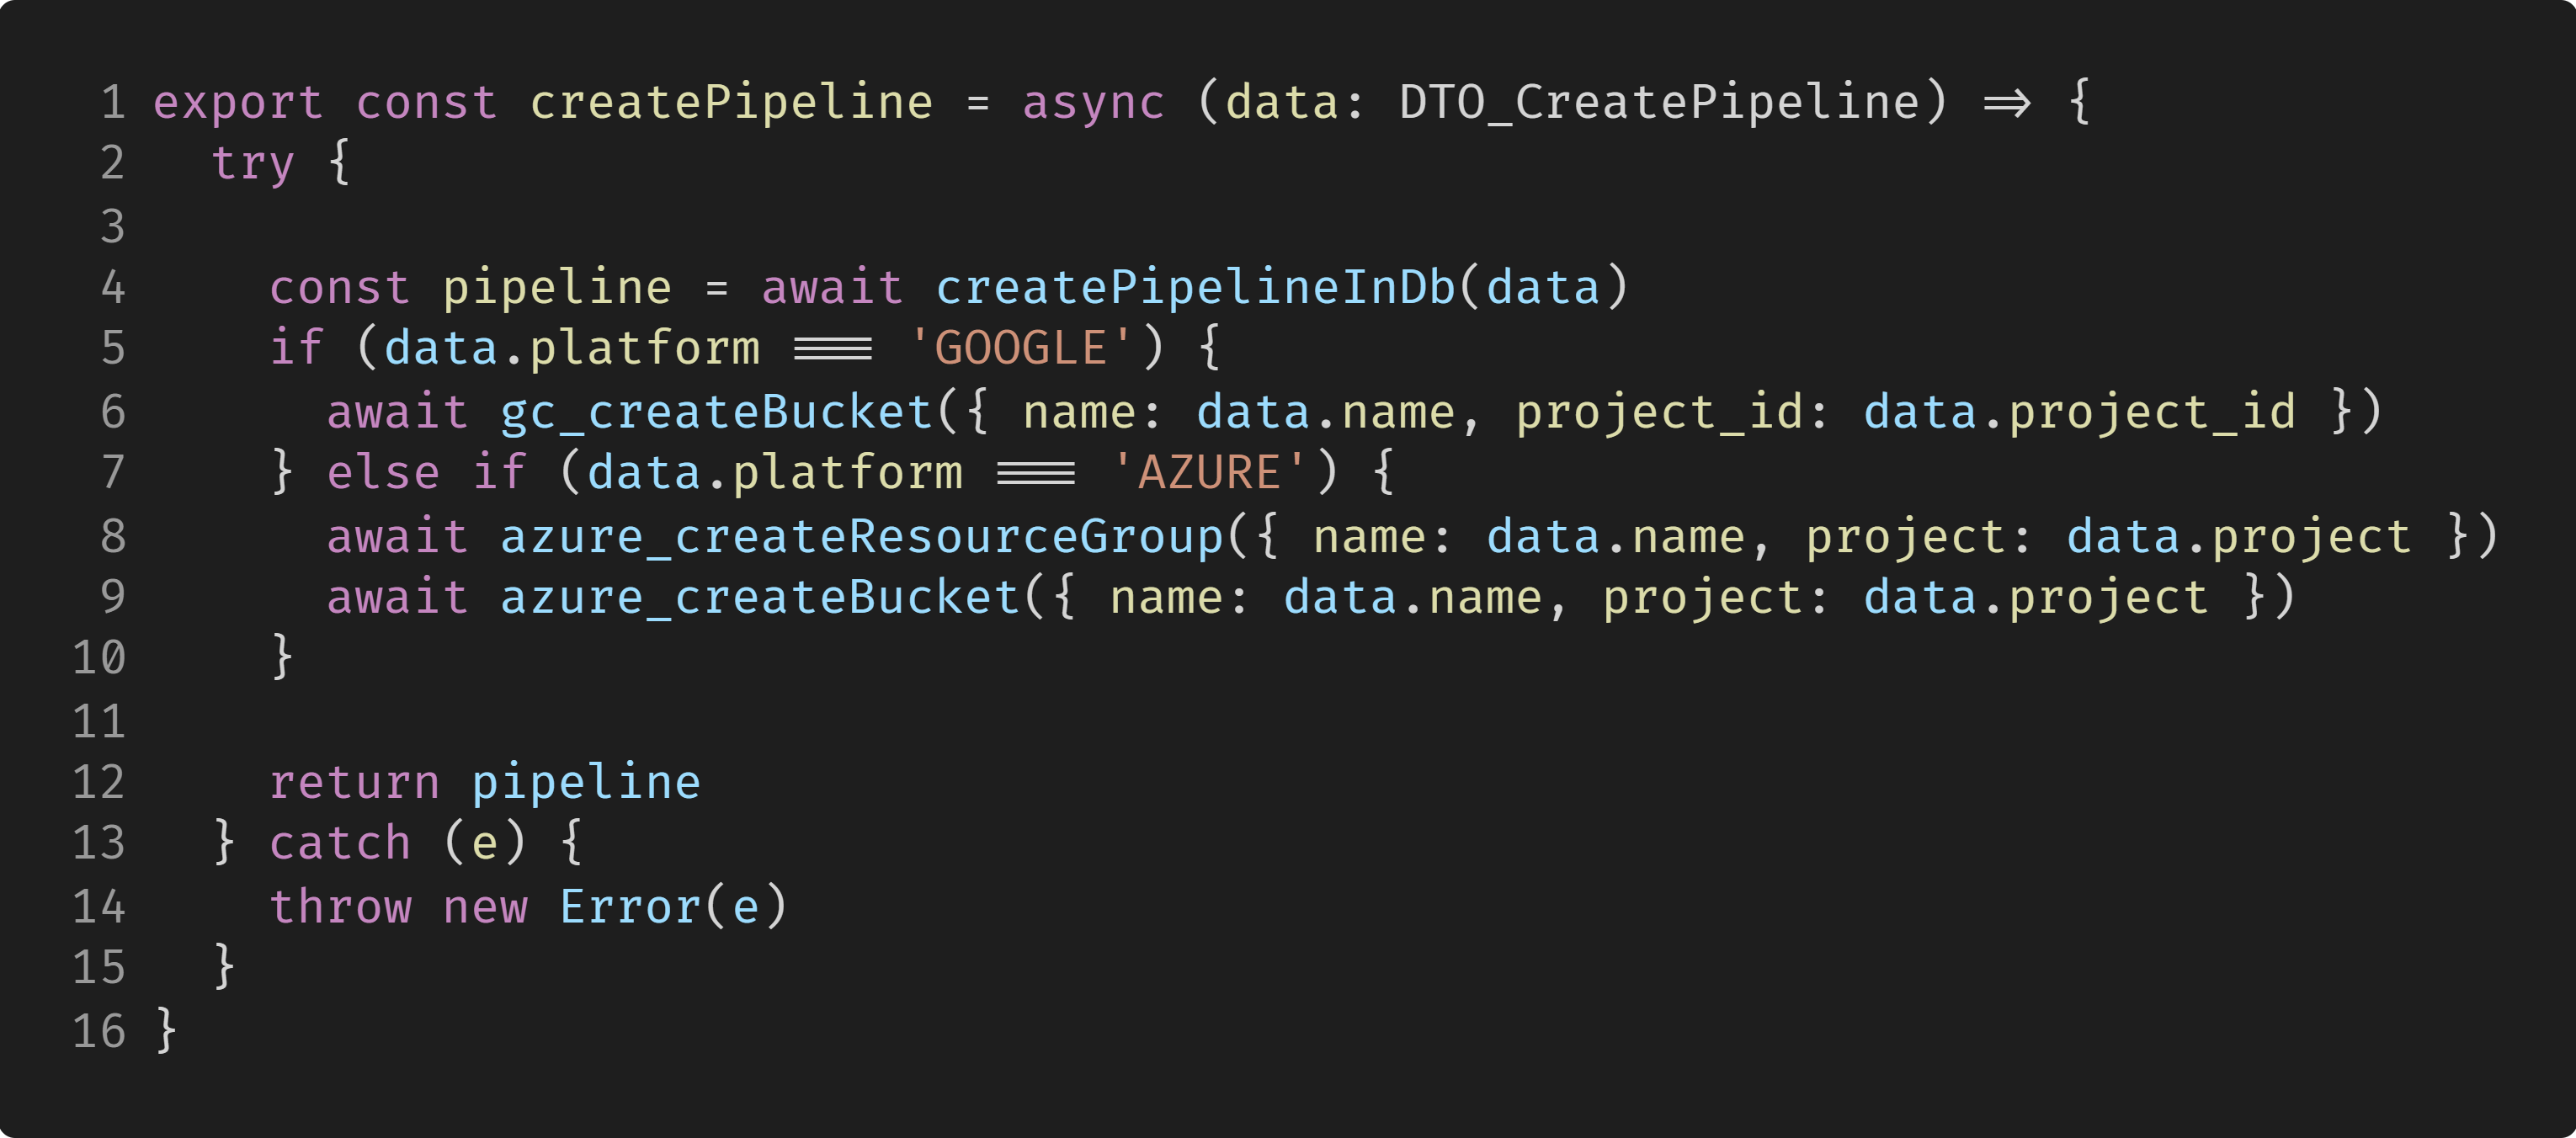
\includegraphics[width=0.85\textwidth]{chapter-7/poc-create-pipeline-service.png}
  \caption{Service om een pipeline aan te maken.}
  \label{fig:ch7-create-pipeline-service}
\end{figure}

Om een pipeline in Google Cloud aan te maken hoeft alleen een storage bucket aangemaakt te worden. De functie die deze actie uitvoert is te zien in \autoref{fig:ch7-create-pipeline-google-cloud}. De bucket heeft een naam nodig en de locatie. Op lijn 5 van \autoref{fig:ch7-create-pipeline-google-cloud} is \textbf{EUROPE-WEST4} gespecificeerd. Dit is een locatie in Nederland.

\begin{figure}[hbt!]
  \centering
  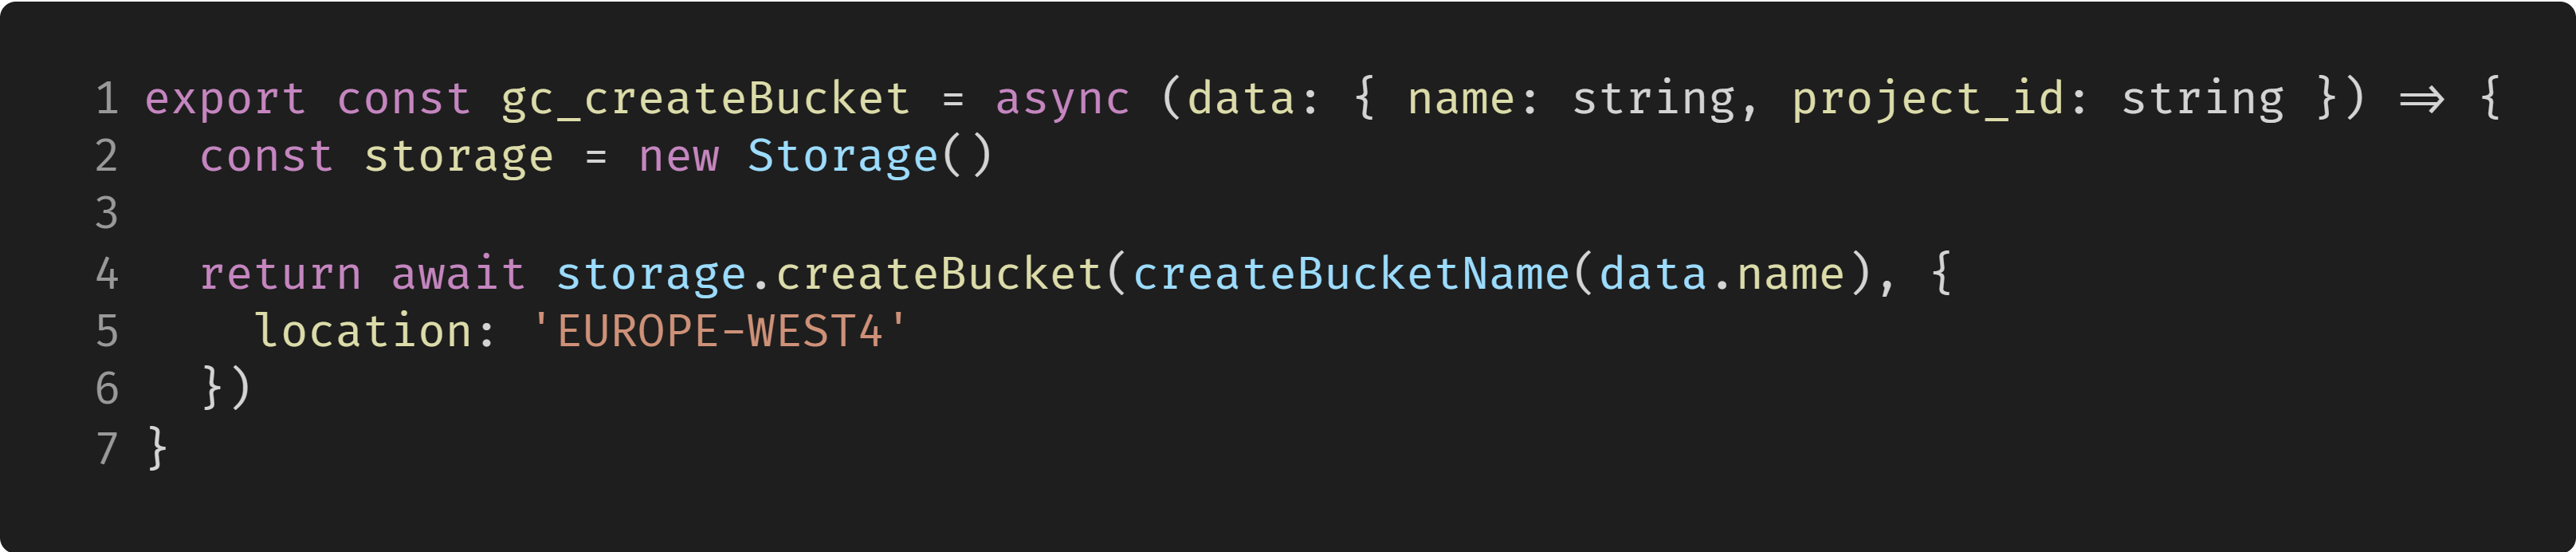
\includegraphics[width=0.9\textwidth]{chapter-7/poc-create-pipeline-google-cloud.png}
  \caption{Functie om een storage bucket aan te maken in Google Cloud.}
  \label{fig:ch7-create-pipeline-google-cloud}
\end{figure}

Naast het aanmaken van de storage bucket in Google Cloud wordt de details van de pipeline opgeslagen in de PostgreSQL database (\autoref{fig:ch7-create-pipeline-service}, lijn 4). Na het aanmaken van een pipeline kan een dataset geüpload worden.

\subsection{Datasets uploaden}\label{subsec:ch7-datasets-uploaden}
Tijdens het aanmaken van de pipeline is een opslaglocatie in de cloud platform aangemaakt. In details weergave van een pipeline is een sectie weergegeven zoals in \autoref{fig:ch7-poc-upload-dataset} waar de developer datasets kan uploaden. Na het uploading krijgt de developer een confirmatie te zien en wordt de lijst met bestaande datasets en artefacts ververst.

\newpage

\begin{figure}[hbt!]
  \centering
  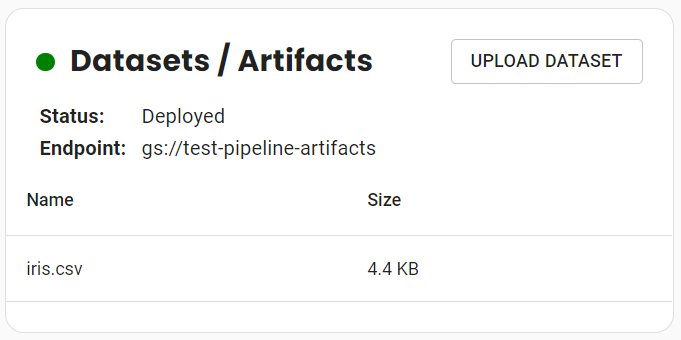
\includegraphics[width=0.9\textwidth]{chapter-7/poc-upload-dataset.png}
  \caption{Status en upload-mogelijkheid van datasets en artefacts in de details pagina van een pipeline.}
  \label{fig:ch7-poc-upload-dataset}
\end{figure}

De code in de backend voor het uploaden is vergelijkbaar met de code in \autoref{fig:ch7-create-pipeline-service} en \autoref{fig:ch7-create-pipeline-google-cloud}. In \autoref{fig:ch7-poc-upload-dataset-service} is de service te zien dat wordt wordt gebruikt als de developer een dataset upload in de frontend. De service selecteert de juiste functie om de dataset te uploaden om basis van het gekozen platform.

\begin{figure}[hbt!]
  \centering
  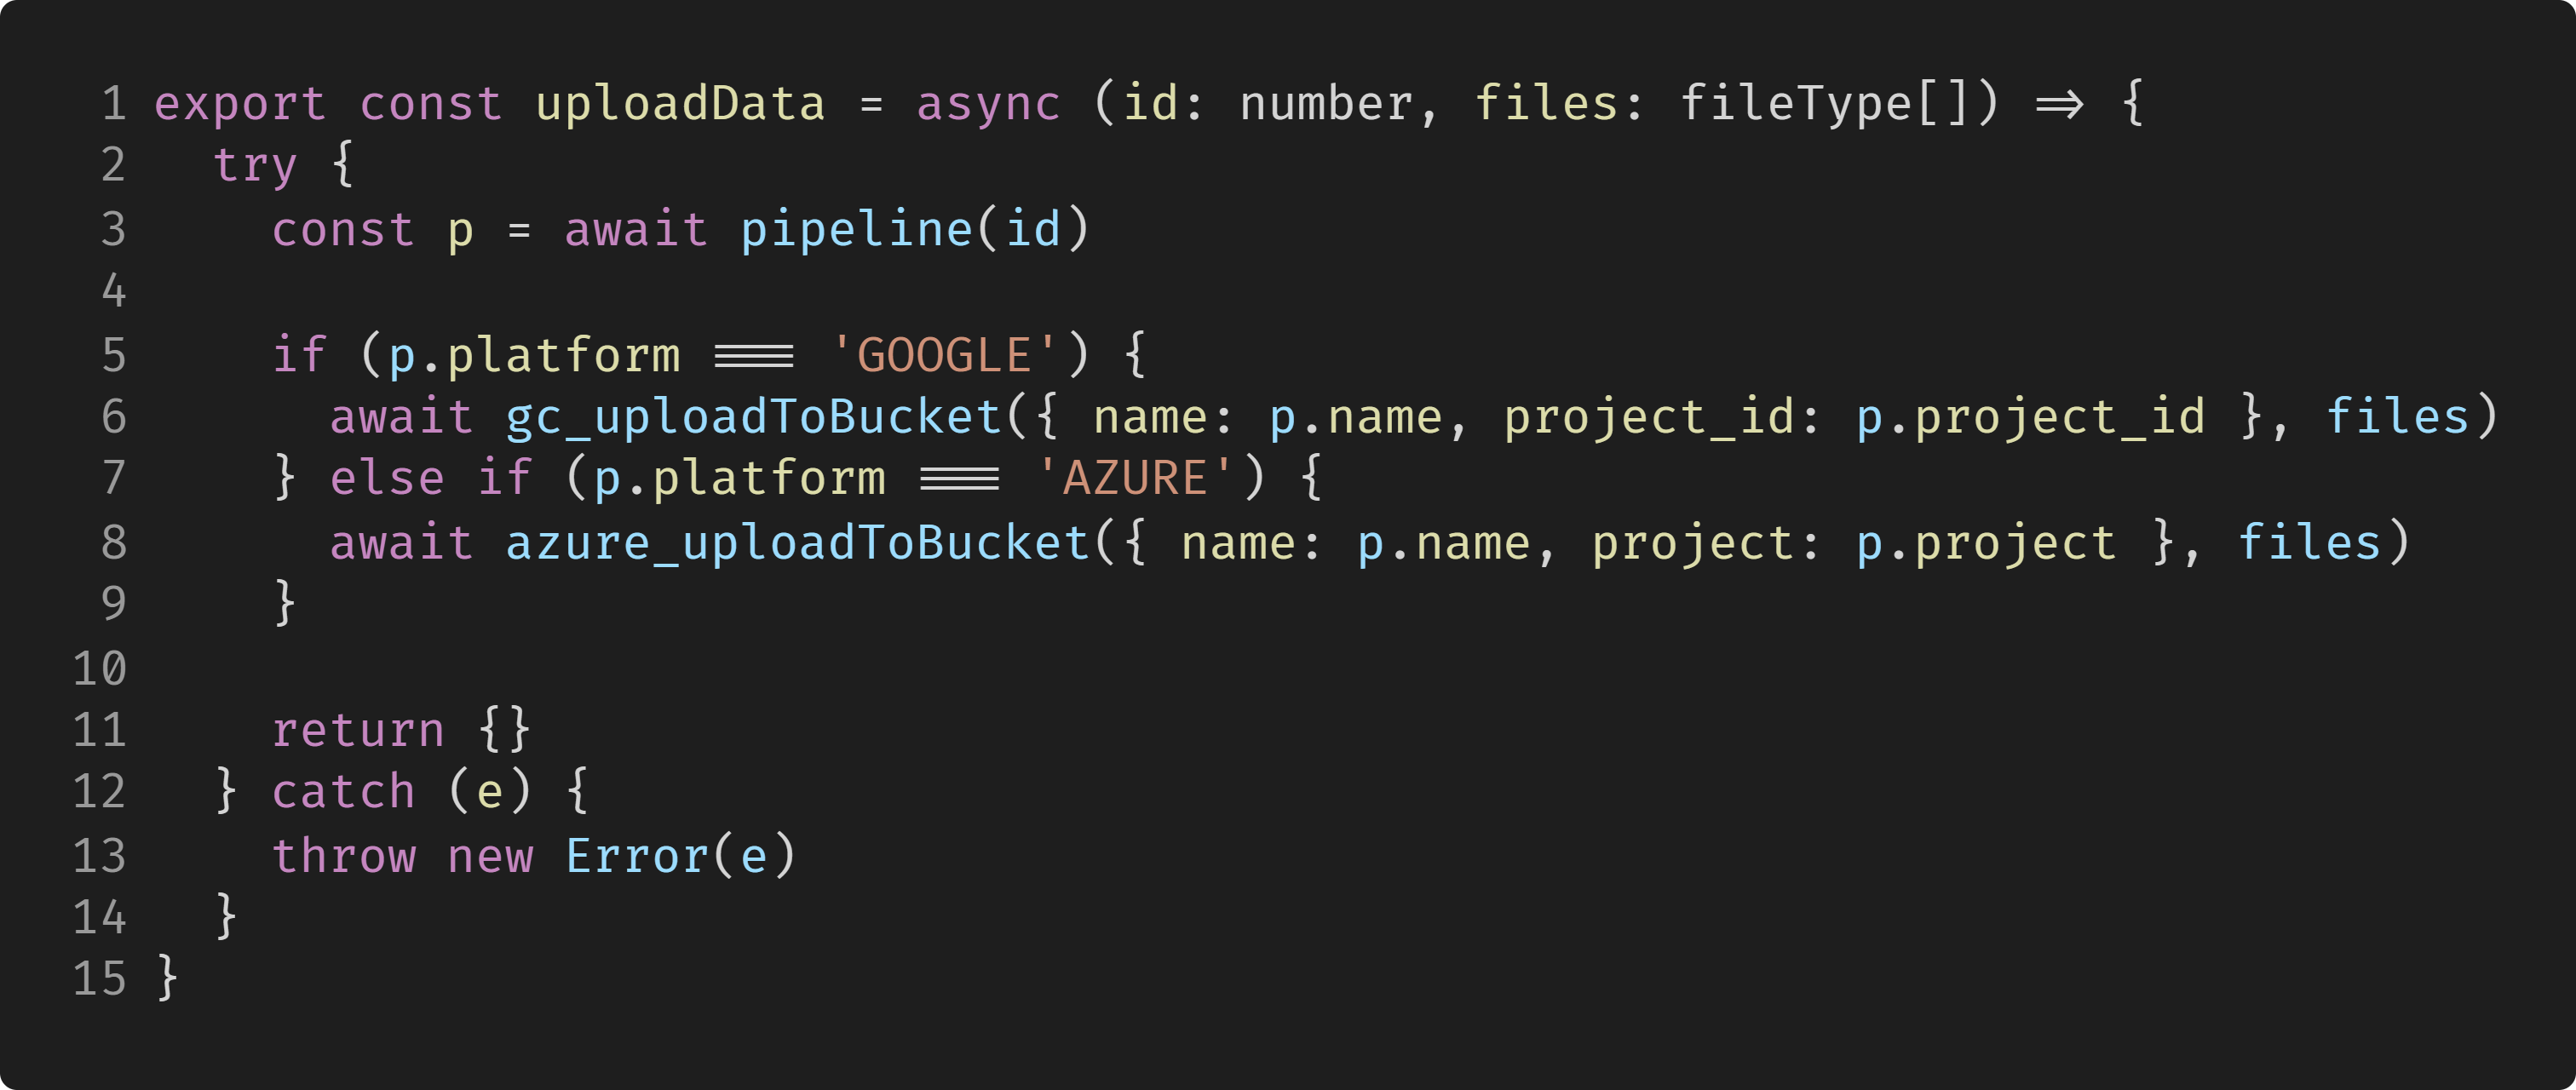
\includegraphics[width=0.8\textwidth]{chapter-7/poc-upload-dataset-service.png}
  \caption{Service om datasets te uploaden naar een opslaglocatie binnen een cloud platform.}
  \label{fig:ch7-poc-upload-dataset-service}
\end{figure}

\newpage

\begin{figure}[hbt!]
  \centering
  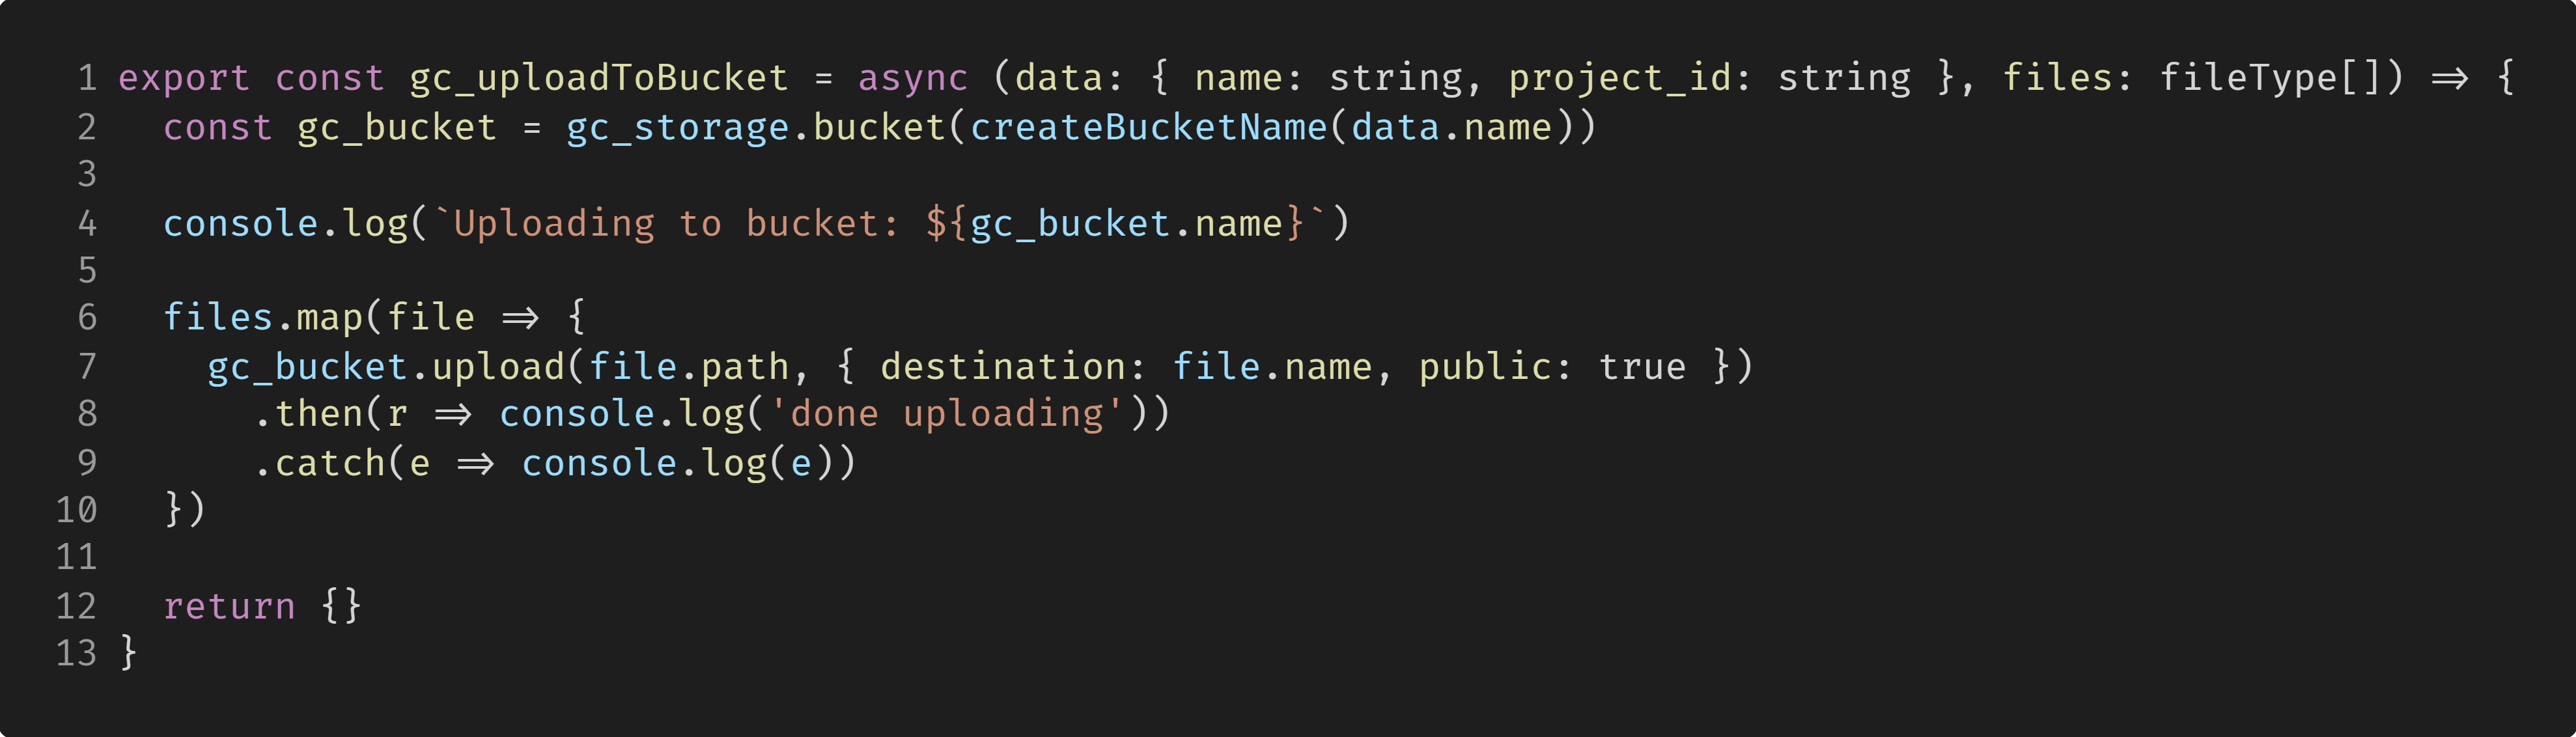
\includegraphics[width=0.9\textwidth]{chapter-7/poc-upload-dataset-google-cloud.png}
  \caption{Functie om datasets te uploaden naar een storage bucket in Google Cloud.}
  \label{fig:ch7-poc-upload-dataset-google-cloud}
\end{figure}

De backend maakt een instantie van de bucket in \autoref{fig:ch7-poc-upload-dataset-google-cloud} op lijn 2 en voert de \(upload()\) functie uit op lijn 7. De geüploade datasets zijn vervolgens beschikbaar om te gebruiken in de configuratie van de pipeline.

\subsection{Configuratie definiëren}\label{subsec:ch7-configuratie-definieren}
Het laatste wat de developer moet doen om de pipeline te starten is het opgeven van de configuratie. Zoals aangegeven in \autoref{sec:ch7-mock-up-van-de-proof-of-concept} is de configuratie een Python bestand dat uitgevoerd wordt als de pipeline gestart wordt. In de PoC is de configuratie bewerkbaar door middel van een dialoog (\autoref{fig:ch7-poc-configuration-dialog}) met rechts een lijst van de datasets. De standaard configuratie dient als startpunt voor de developer. Een link naar de dataset kan gekopieerd worden door op een dataset te klikken.

\begin{figure}[hbt!]
  \centering
  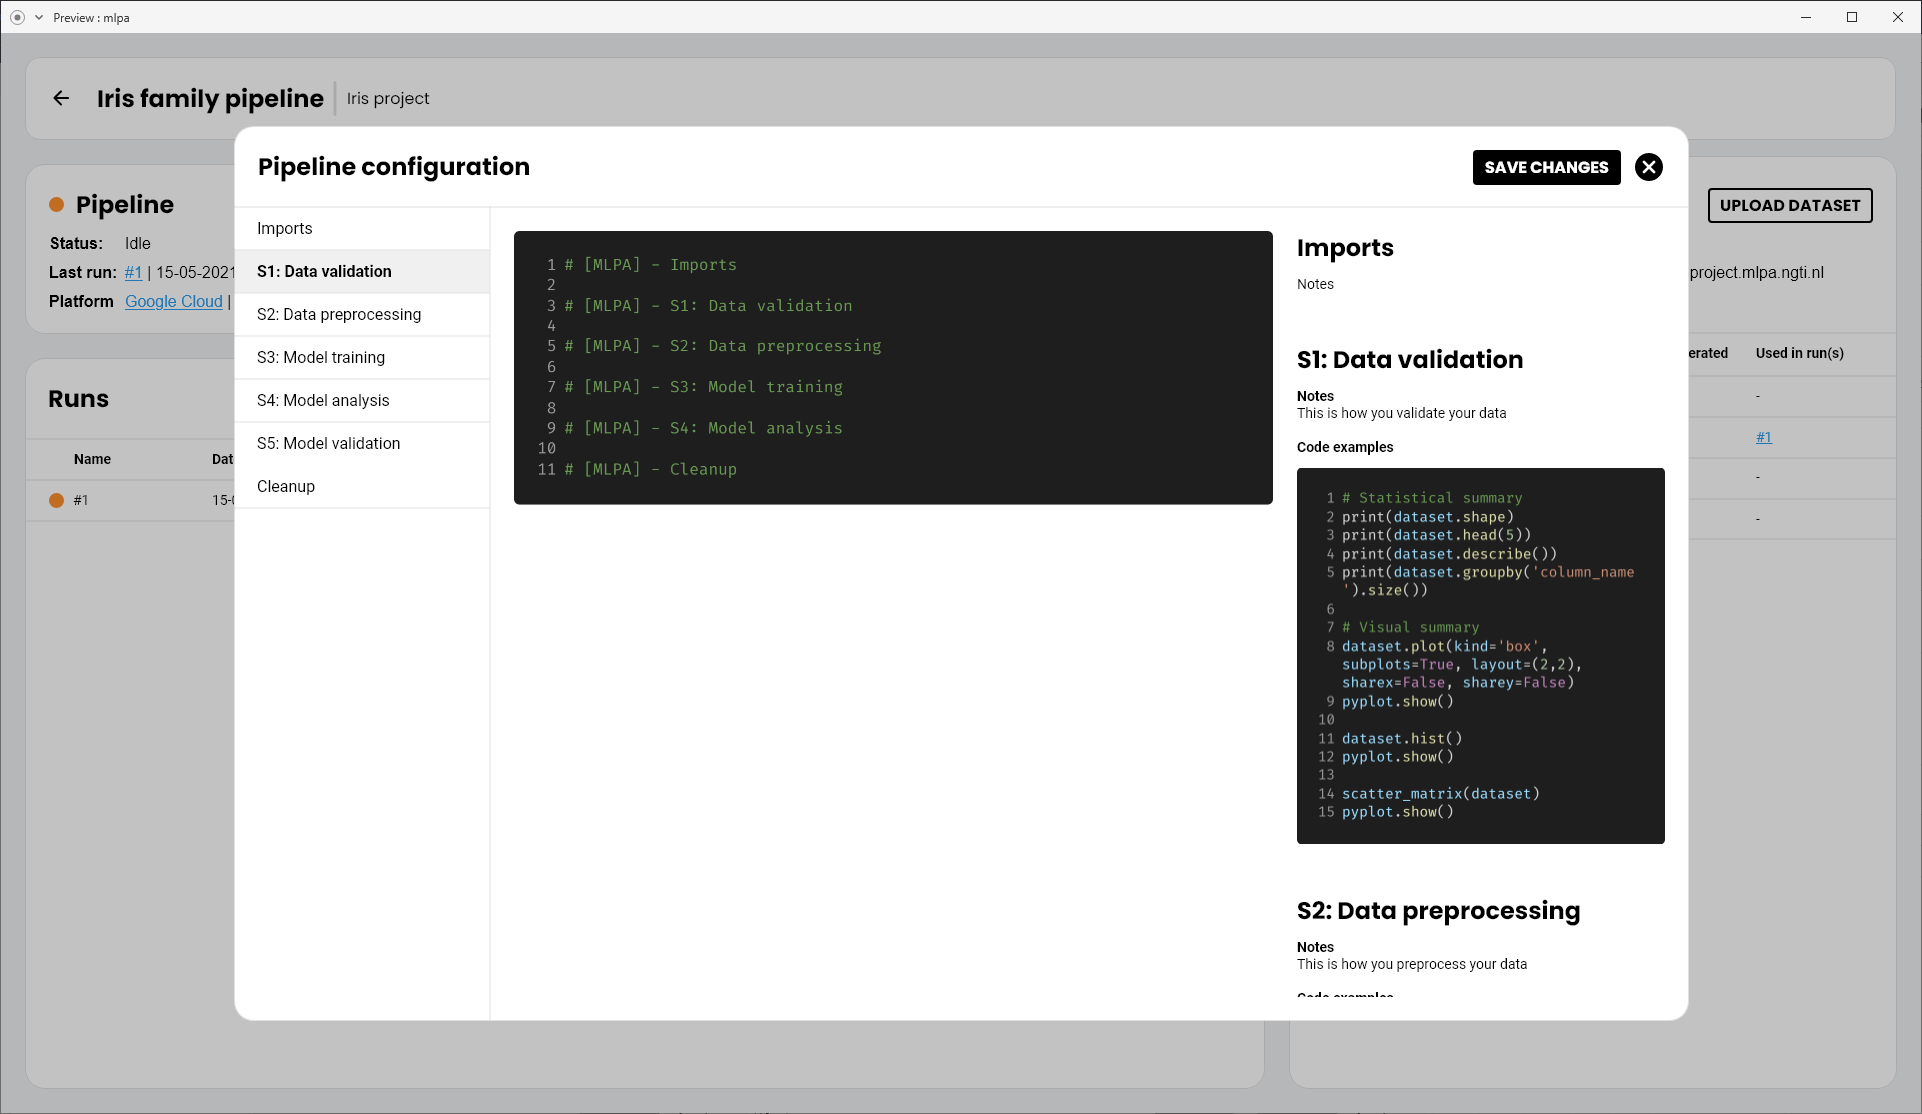
\includegraphics[width=0.9\textwidth]{chapter-7/poc-configuration-dialog.png}
  \caption{Configuratie dialoog van een pipeline.}
  \label{fig:ch7-poc-configuration-dialog}
\end{figure}

Zodra de developer op de knop \textbf{SAVE} klikt, wordt een request gedaan naar de backend om de configuratie op te slaan. De code om de configuratie op te slaan is te zien in \autoref{fig:ch7-poc-configuration-commit-db}. Hier wordt een nieuwe configuratie aangemaakt en gelinkt aan de pipeline.

\begin{figure}[hbt!]
  \centering
  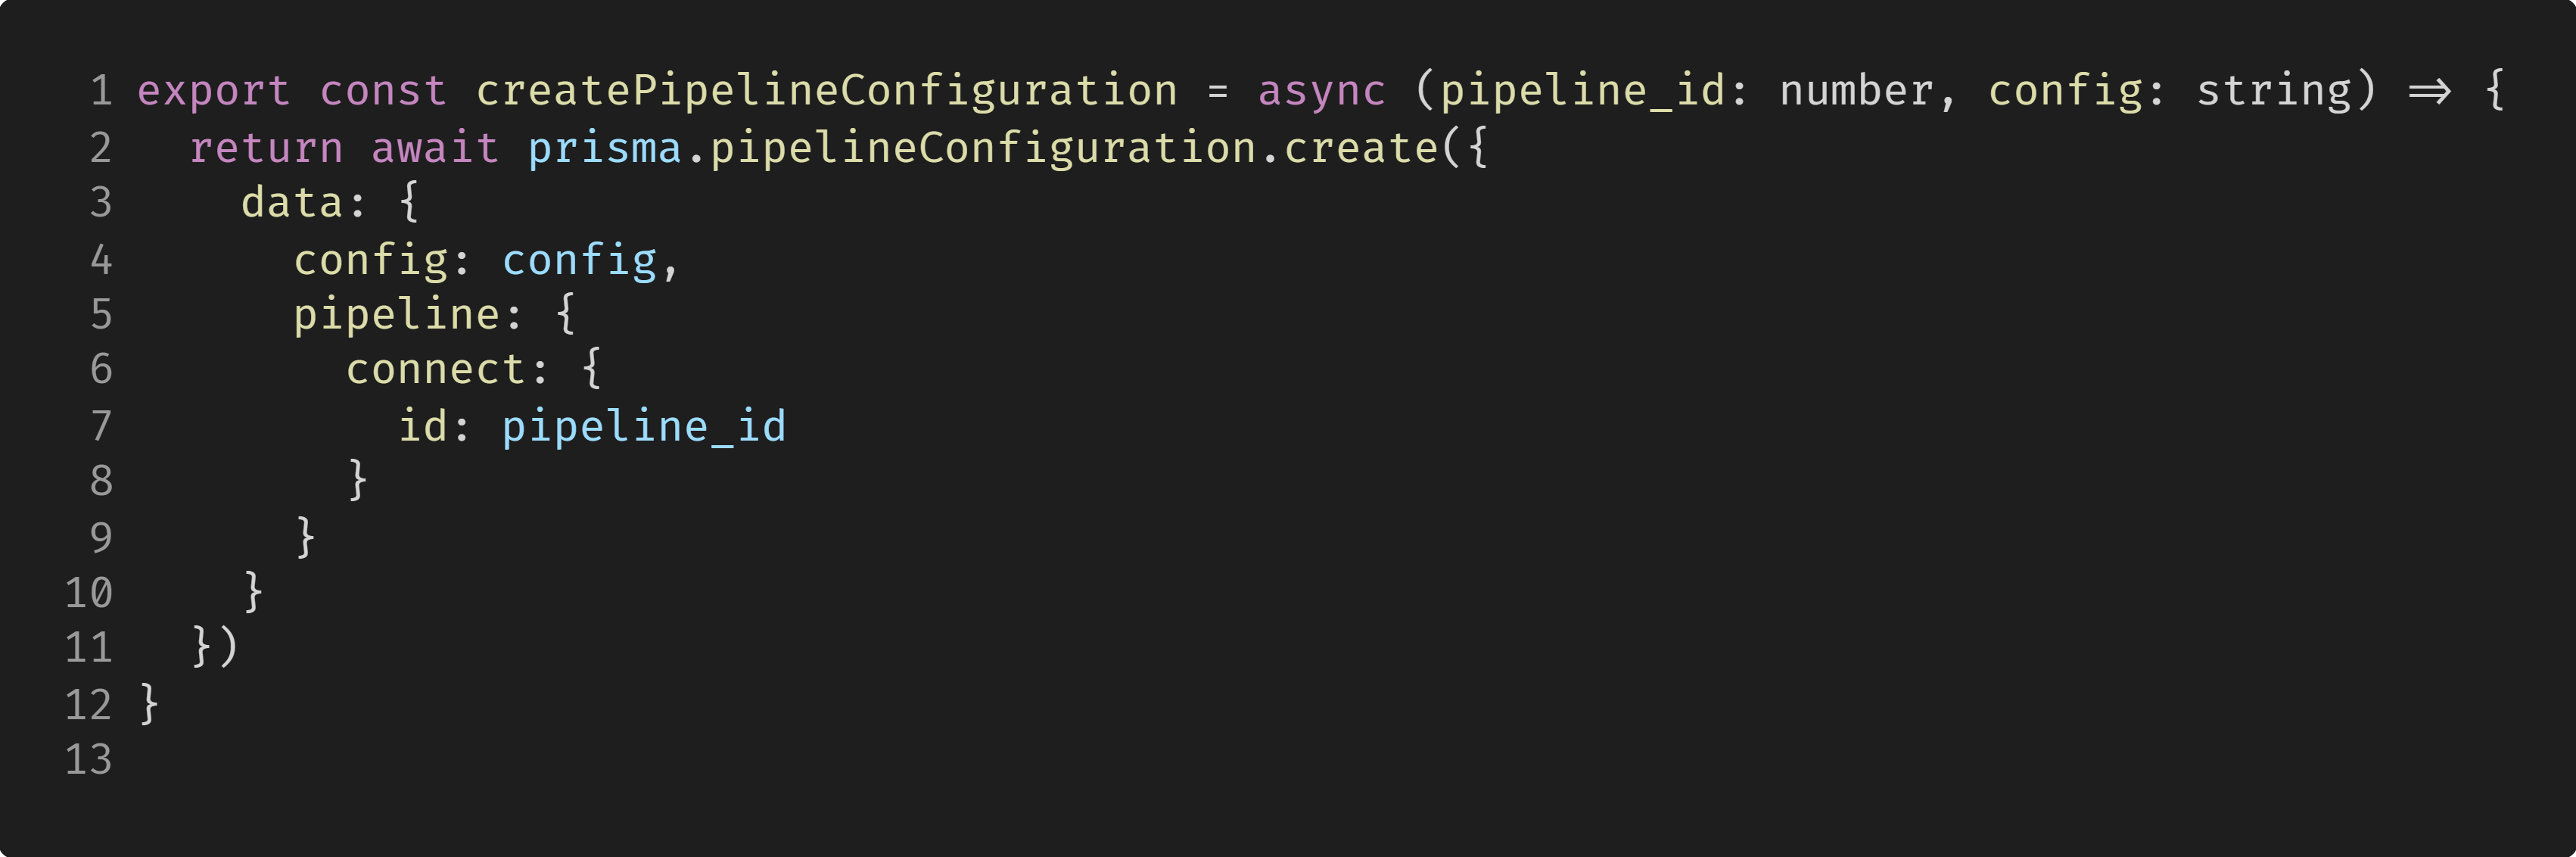
\includegraphics[width=0.85\textwidth]{chapter-7/poc-configuration-commit-db.png}
  \caption{Code om de configuratie op te slaan in de database.}
  \label{fig:ch7-poc-configuration-commit-db}
\end{figure}

Het is mogelijk om code te schrijven in andere talen dan Python om modellen te trainen. Om de complexiteit en scope klein en realistisch te houden is er gekozen voor Python. De taal is een van de populairste talen \cite{stack-overflow-survey-2020-loved-dreaded-framework-libraries-tools}. Daarnaast heeft Python een complete set van libraries om data te transformeren, plotten in diagrammen en modellen te trainen \cite{python-libraries}. Nu de configuratie is opgeslagen zijn alle benodigdheden beschikbaar om de pipeline te starten. 

\subsection{Pipeline starten}\label{subsec:ch7-pipeline-starten}
Zodra de opslaglocatie en configuratie beschikbaar zijn, krijgt de developer de mogelijkheid om de pipeline te starten \autoref{fig:ch7-poc-start-pipeline}. Zoals uitgelegd in \autoref{fig:ch6-c4-sd-start-pipeline} worden drie stappen uitgevoerd: het aanmaken van een \acrshort{vm}, het continu ophalen van de output en vervolgens het verwijderen van de \acrshort{vm}.

\begin{figure}[hbt!]
  \centering
  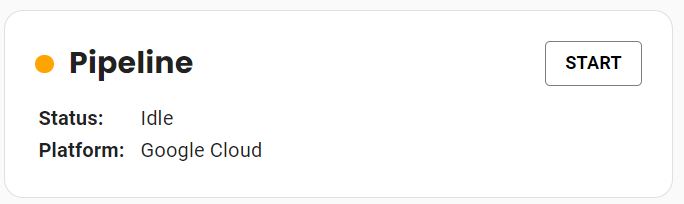
\includegraphics[width=0.45\textwidth]{chapter-7/poc-start-pipeline.png}
  \caption{Status en startknop van een pipeline.}
  \label{fig:ch7-poc-start-pipeline}
\end{figure}

De request van de frontend komt in de backend binnen om een pipeline te starten en komt terecht bij de functie \(gc\_startPipeline()\) in \autoref{fig:ch7-poc-start-pipeline-google-cloud}. Deze functie maakt een configuratie aan op lijn 7 waarin de besturingssysteem, soort \acrshort{vm} in Google Cloud en de start-up script staat gedefinieerd. De configuratie wordt gebruikt als de \acrshort{vm} wordt aangemaakt op lijn 27. De status van de pipeline wordt aangepast naar \textbf{"RUNNING"} en een nieuwe Run wordt aangemaakt in het database.

\begin{figure}[hbt!]
  \centering
  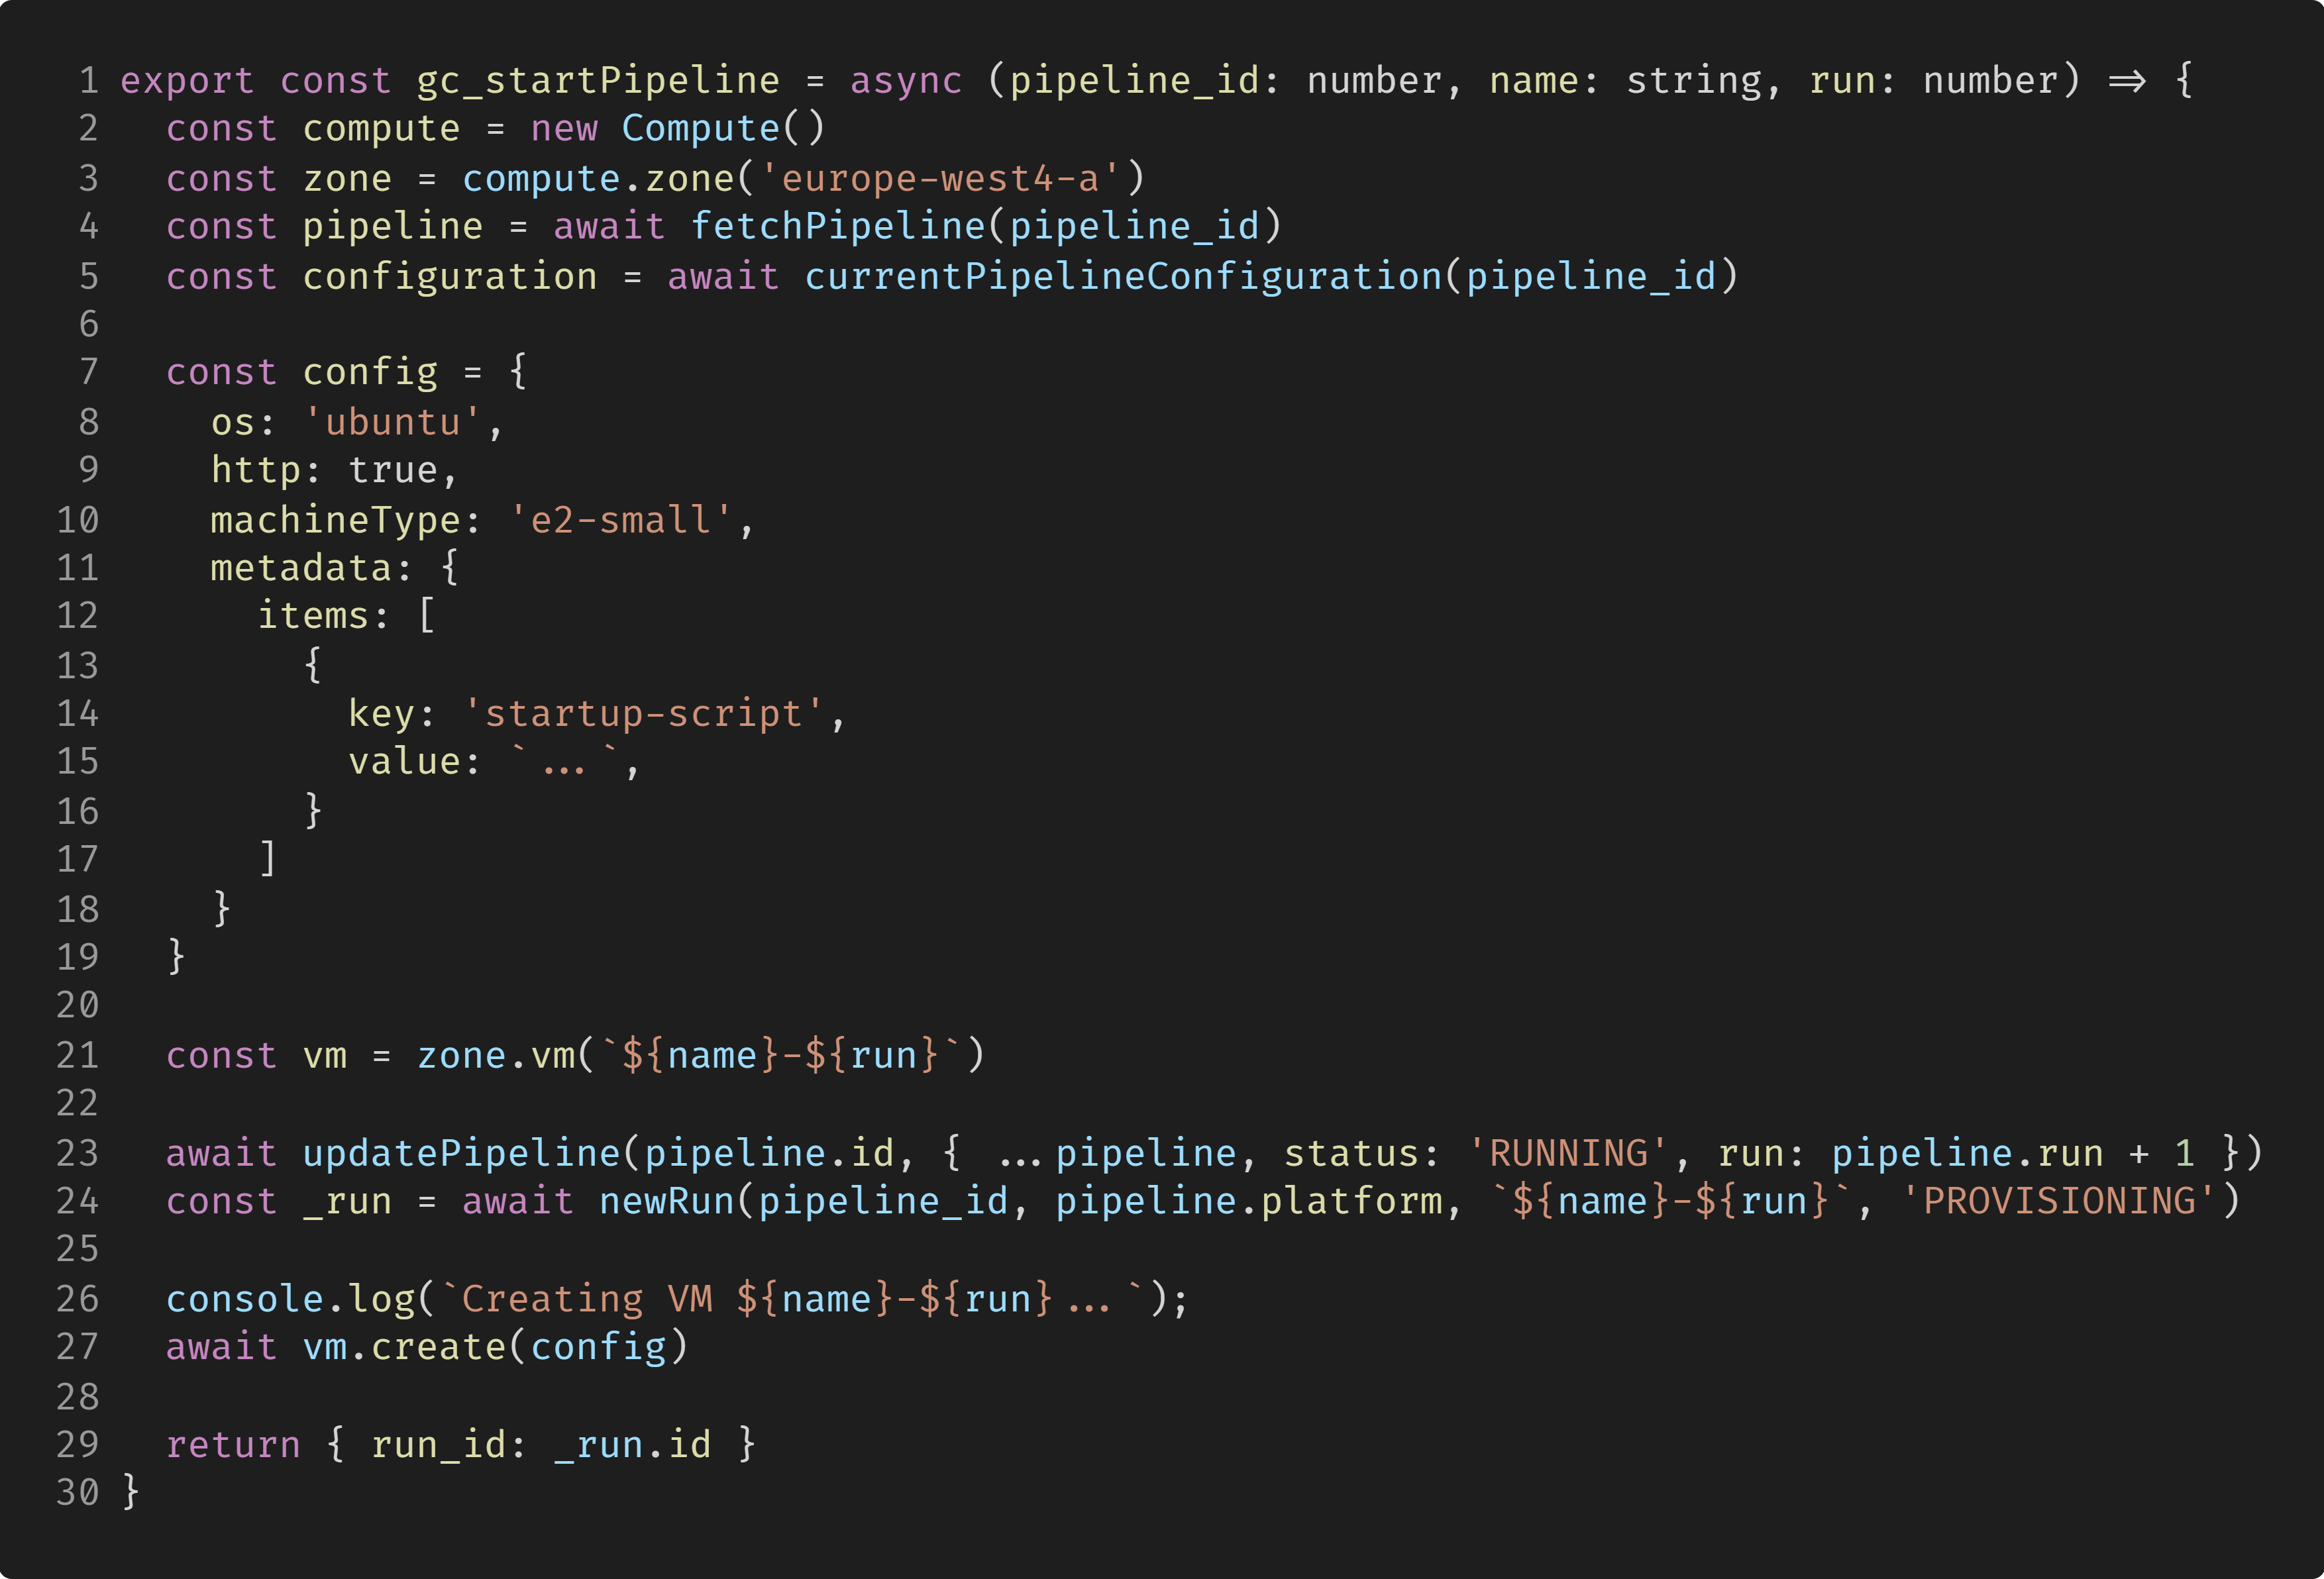
\includegraphics[width=.8\textwidth]{chapter-7/poc-start-pipeline-google-cloud.png}
  \caption{Code om een \acrfull{vm} in Google Cloud te starten.}
  \label{fig:ch7-poc-start-pipeline-google-cloud}
\end{figure}

\newpage

In de configuratie is een start-up script gedefinieerd (\autoref{fig:ch7-poc-start-pipeline-google-cloud}, lijn 15). De script wordt uitgevoerd zodra de \acrshort{vm} beschikbaar is en zorgt ervoor dat het model getraind kan worden en \glspl{artifact} opgeslagen worden in de opslaglocatie indien dit nodig is. Op lijn 18 in \autoref{fig:ch7-poc-start-pipeline-config-google-cloud} wordt de configuratie die de developer heeft opgeslagen in \autoref{subsec:ch7-configuratie-definieren} in het script gezet. Na het trainen van het model worden alle \glspl{artifact} in de \(output\) map geüpload naar de opslaglocatie. Dit gebeurt met bash commando's op lijn 34 en 35.

\newpage

\begin{figure}[hbt!]
  \centering
  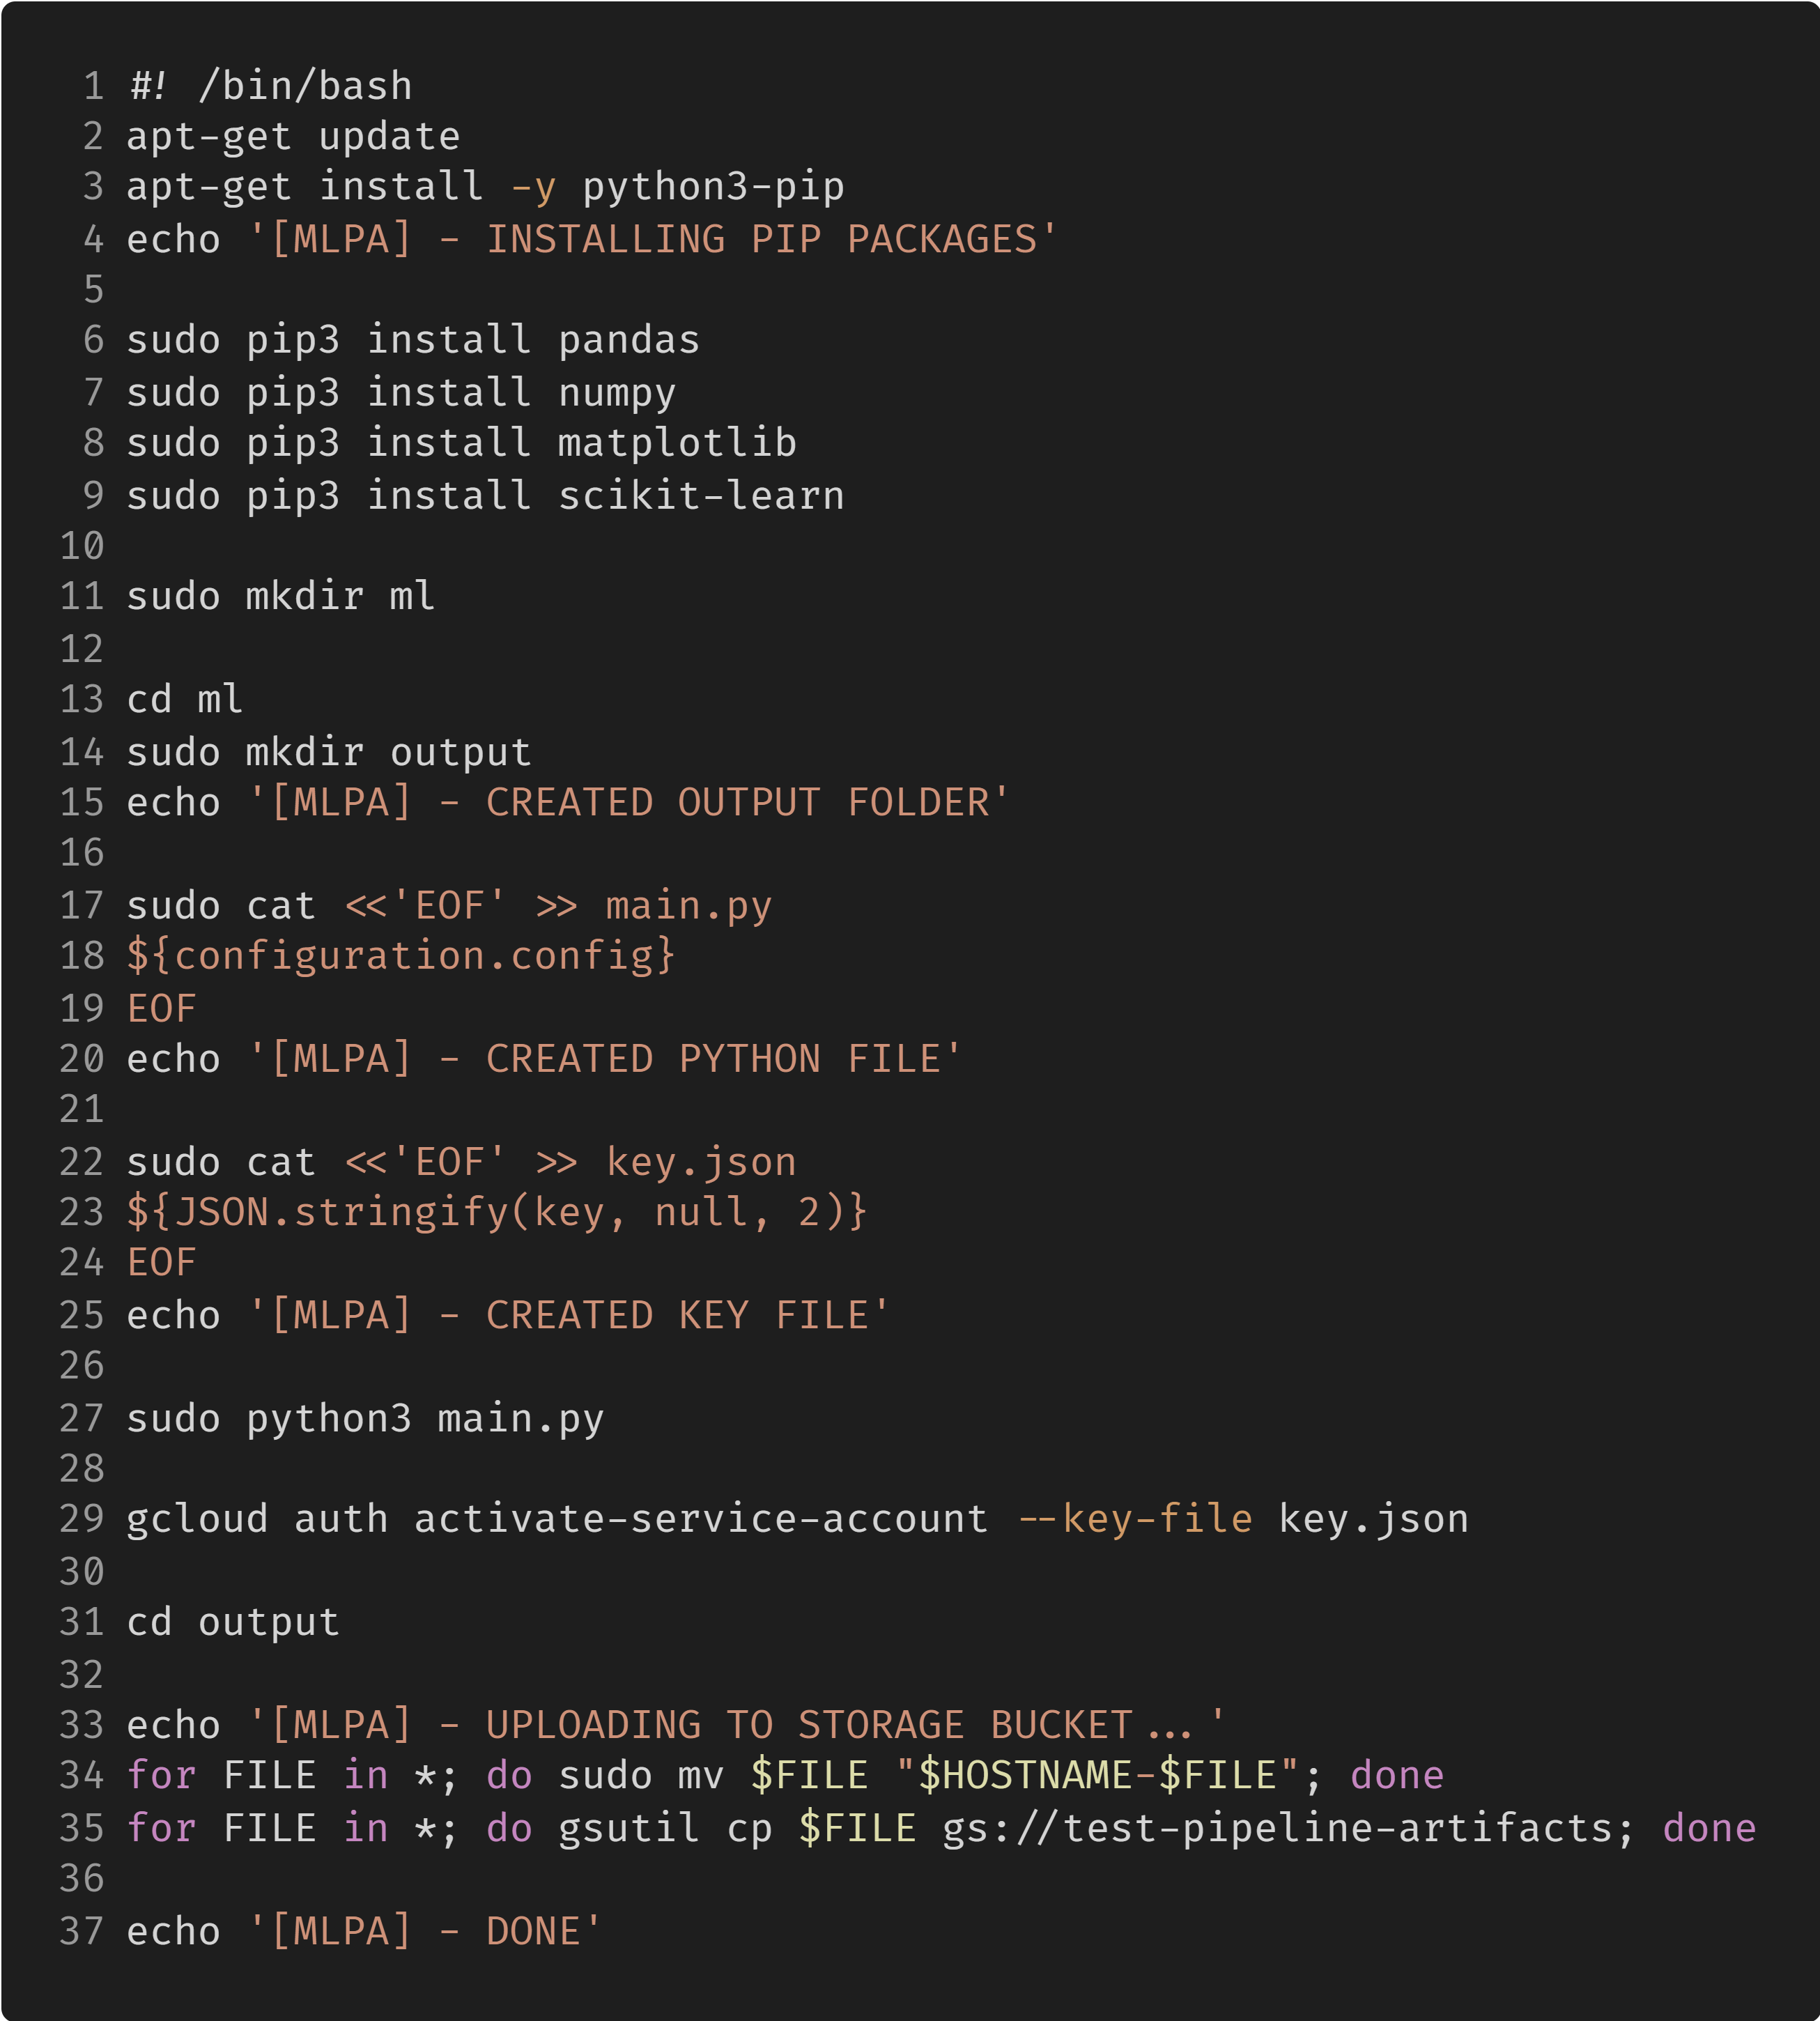
\includegraphics[width=.75\textwidth]{chapter-7/poc-start-pipeline-config-google-cloud.png}
  \caption{Start-up script van een \acrfull{vm} in Google Cloud.}
  \label{fig:ch7-poc-start-pipeline-config-google-cloud}
\end{figure}

Gedurende het uitvoeren van de script in \autoref{fig:ch7-poc-start-pipeline-google-cloud} vraagt de frontend continu naar de output van de \acrshort{vm}. Deze request wordt afgehandeld door de \(gc\_getRunStatus()\) functie in bijlage \ref{appendix:poc-get-run-status}. De functie haalt de output op (lijn 9) en slaat het op in de database voordat het terug gestuurd wordt naar de frontend. De frontend laat de output zien (bijlage \ref{appendix:poc-vm-output-google-cloud}) en controleert of de output \textbf{'[MLPA] - DONE'} bevat. Als de output deze tekst bevat, weet het systeem dat het model is getraind en alle \glspl{artifact} in de output map geüpload zijn in de opslaglocatie. Als dit niet het geval is, wordt de output opnieuw opgehaald en geüpdatet in de frontend. Dezelfde controle op de output vindt vervolgens weer plaats. Als de output wel \textbf{'[MLPA] - DONE'} bevat, wordt er middels een request aan de backend de \acrshort{vm} verwijderd (bijlage \ref{appendix:poc-destroy-vm}). In het verwijderproces wordt de status in de database geüpdatet.

\subsection{Model downloaden}\label{subsec:ch7-model-downloaden}
Nadat het model getraind is, worden \glspl{artifact} in de \(output\) map geüpload naar de opslaglocatie. Het is aan de developer om in het Python script te definiëren dat artifacts opgeslagen worden in de \(output\) map. De lijst met datasets/\glspl{artifact} wordt geüpdatet zodra de start-up script klaar is. De \glspl{artifact} zijn downloadbaar door erop te klikken.

\begin{figure}[hbt!]
  \centering
  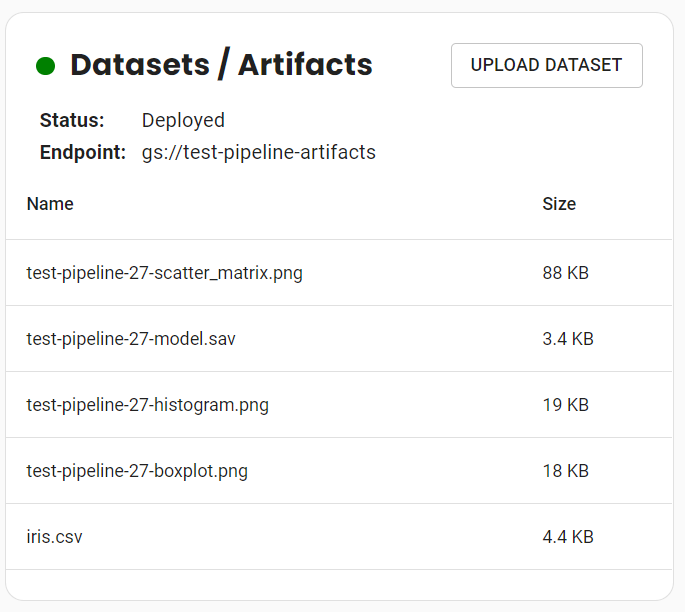
\includegraphics[width=.5\textwidth]{chapter-7/poc-datasets-and-artifacts-after-training.png}
  \caption{Model en overige \glspl{artifact} van het trainproces geüpload in een storage bucket.}
  \label{fig:ch7-poc-datasets-and-artifacts-after-training}
\end{figure}

\section{Kwaliteit van de code}\label{sec:ch7-kwaliteit-van-de-code}
Gedurende het ontwikkelproces is gebruik gemaakt van de repository-service pattern, verschillende principes en "good practices". In \autoref{sec:ch6-architecturaal-ontwerp} is de repository-service pattern kort uitgelegd. Het idee achter deze pattern is dat het ophalen van data uit de database en complexe logica gescheiden van elkaar blijft \cite{repository-service-pattern}. De repository laag in \autoref{fig:ch7-repository-service-pattern-example} bevat \acrfull{crud} functies die in verschillende services hergebruikt kan worden. 

\begin{figure}[hbt!]
  \centering
  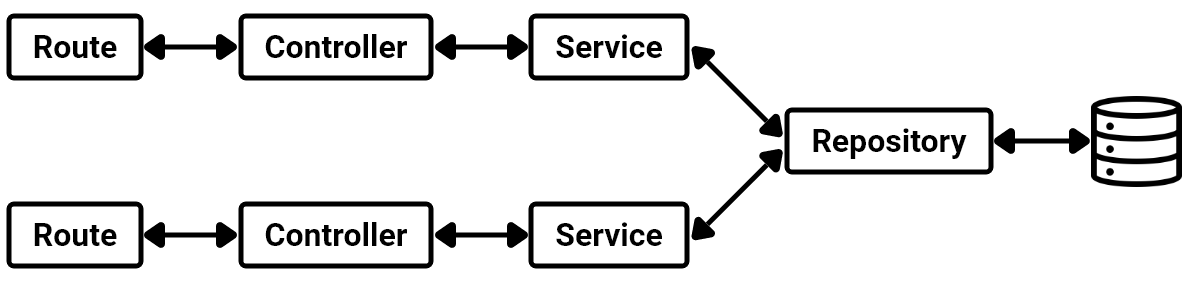
\includegraphics[width=.8\textwidth]{chapter-7/repository-service-pattern-example.png}
  \caption{Voorbeeld van de repository-service pattern.}
  \label{fig:ch7-repository-service-pattern-example}
\end{figure}

Doordat de architectuur ontworpen is met de repository-service pattern, voldoet de PoC ook aan de \acrfull{dry} \cite{clean-code-martin}. Volgens deze principe moet er geen code geschreven worden dat al geschreven is. Functies zoals het ophalen van een pipeline kan hergebruikt worden met behulp van de repository laag (\autoref{fig:ch7-dry-principle-example}).

\newpage

\begin{figure}[hbt!]
  \centering
  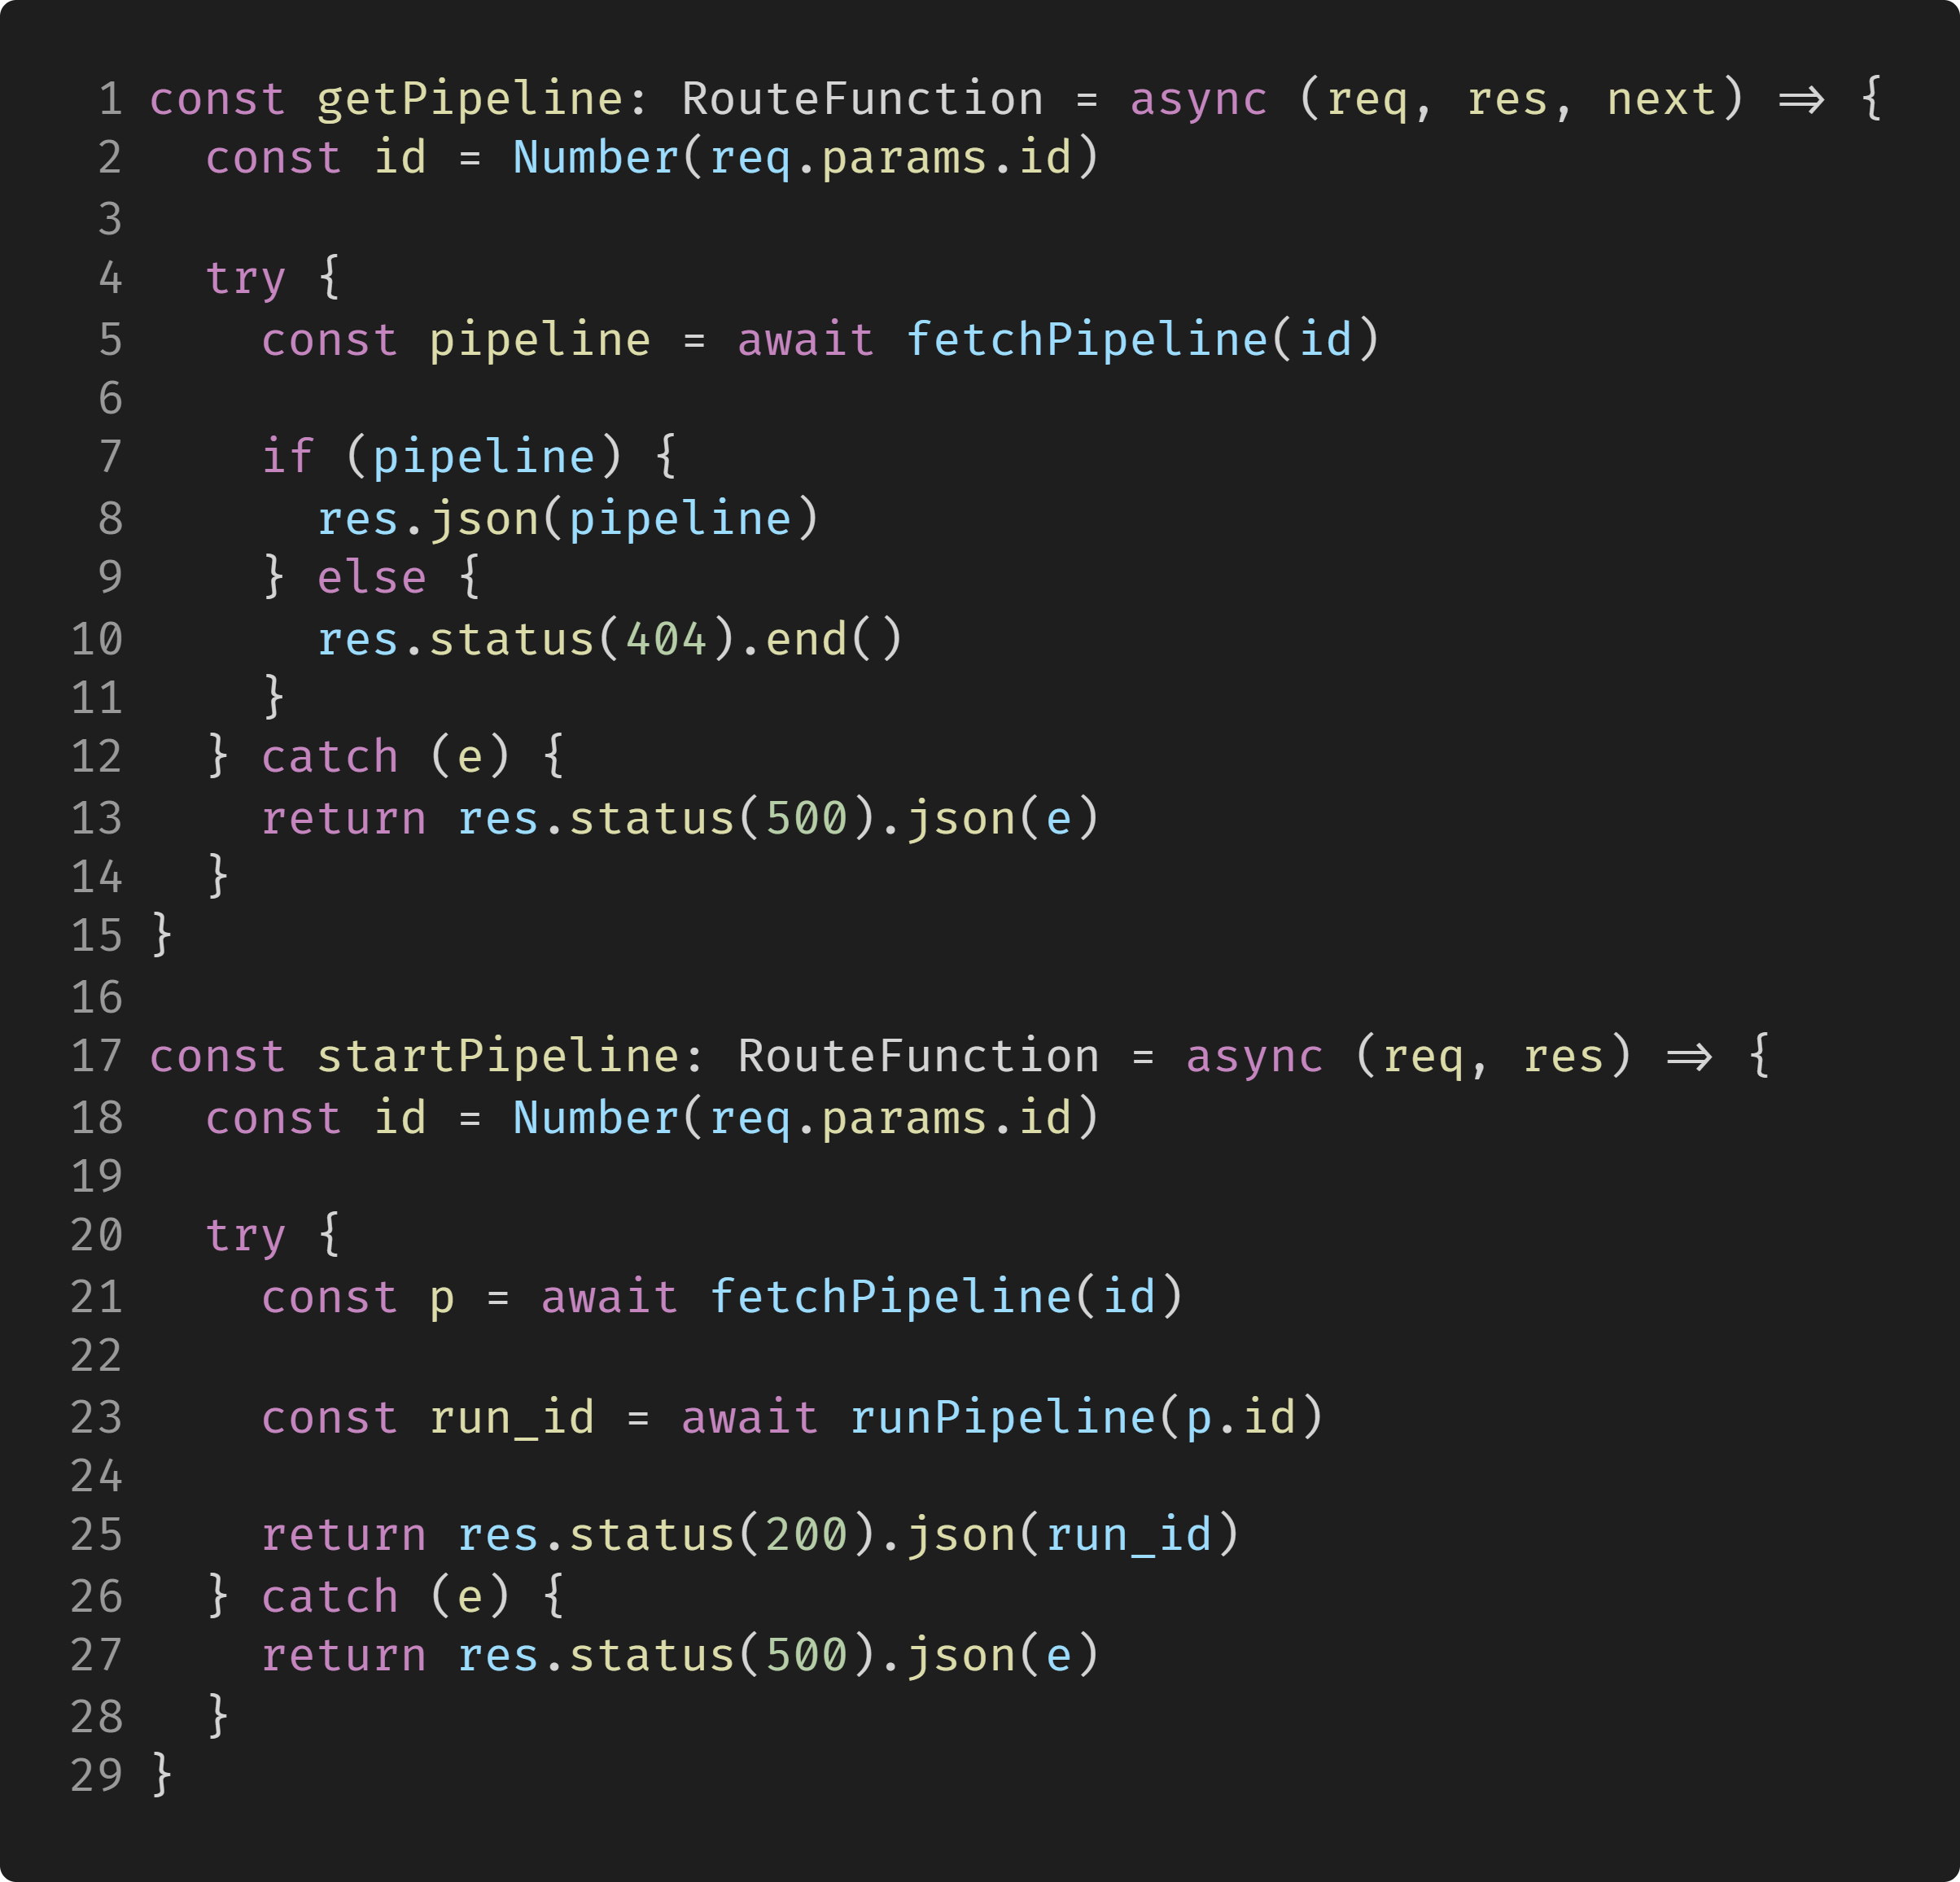
\includegraphics[width=.65\textwidth]{chapter-7/dry-principle-example.png}
  \caption{Voorbeeld van de \acrfull{dry} principe in de backend.}
  \label{fig:ch7-dry-principle-example}
\end{figure}

De toepassing van de \acrshort{dry} principe komt ook voor in de code van de frontend. Zoals weergegeven in \autoref{fig:ch7-frontend-dry-principle-example} wordt bijvoorbeeld de container waar elke sectie in zit hergebruikt. Met deze werkwijze kunnen elementen in de frontend sneller en consistenter gebouwd worden.

\begin{figure}[hbt!]
  \centering
  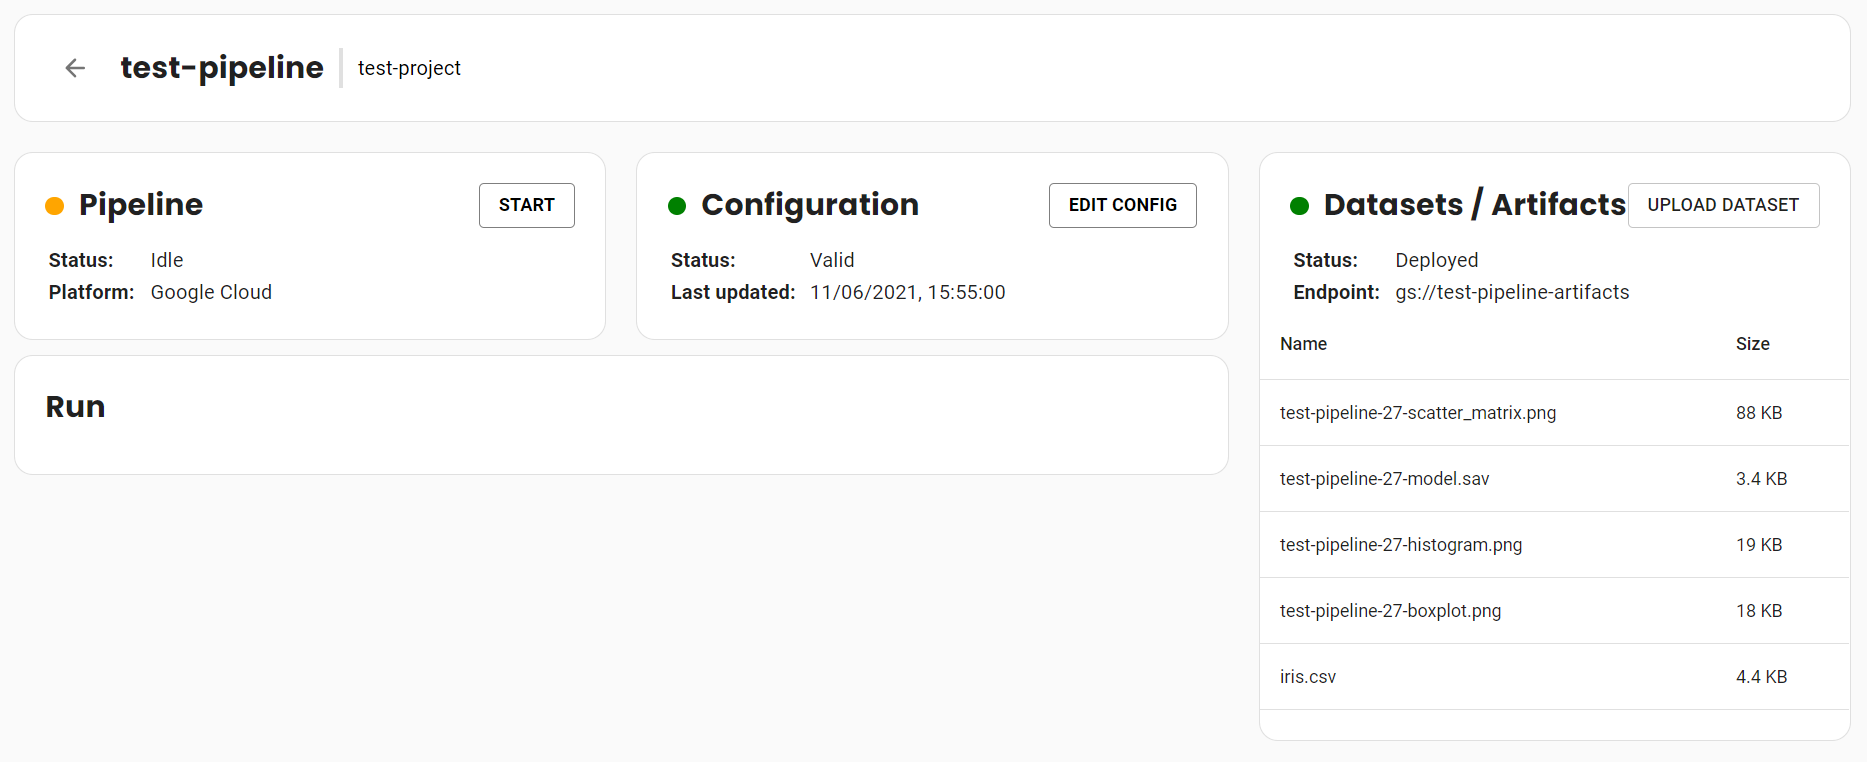
\includegraphics[width=.9\textwidth]{chapter-7/frontend-dry-principle-example.png}
  \caption{Voorbeeld van de \acrfull{dry} principe in de frontend.}
  \label{fig:ch7-frontend-dry-principle-example}
\end{figure}

% ---

\section{Conclusie}\label{sec:ch7-conclusie}
In dit hoofdstuk is onderzoek gedaan naar het antwoord op de hoofdvraag: \textbf{H: In welke mate kan een machine learning pipeline worden geautomatiseerd onafhankelijk van de onderliggende cloud computing platform?} Het onderzoek is uitgevoerd met het verzamelen van requirements, ontwerpen van een mock up en een PoC bouwen.

Middels het implementeren is duidelijk geworden dat een orkestratietool niet de correcte werkwijze is om infrastructuur aan te passen. De tool verwacht dat alle resources, ook resources die voorheen aangemaakt zijn, in het plan zijn gedefinieerd. Resources worden verwijderd als dit het geval is. Om dit op te lossen is gekozen om te werken met libraries van de cloud platformen zelf. Documentatie van de libraries is aanwezig, echter laat documentatie van een aantal libraries te wensen over. De functionaliteit om resources aan te maken is wel aanwezig en is dus een valide vervanging.

De scope van de PoC bevat de stappen uit \autoref{fig:ch4-model-lifecycle-oreilly} om een model te trainen. Het trainen gaat met een Python bestand dat als configuratie wordt opgeslagen. Eerst moet een pipeline aangemaakt worden zodat de PoC de benodigdheden klaar kan zetten voor de developer. Dat is de opslaglocatie in de gekozen cloud platform en informatie over de pipeline in de database. Vervolgens kan de developer een dataset uploaden, de configuratie opslaan en de pipeline starten. Na het starten maakt de PoC een \acrshort{vm} aan in de cloud platform en voert een script uit zodat het model getraind en opgeslagen kan worden samen met overige \glspl{artifact} in de opslaglocatie. Tot slot wordt de \acrshort{vm} verwijderd en is het model beschikbaar om te gebruiken in een webserver of app om voorspellingen of classificaties te maken.

\section{Advies}\label{sec:ch7-advies}
De PoC laat zien dat het automatiseren van een pipeline mogelijk is. Een developer van NGTI heeft alleen kennis nodig van ML om gebruik te maken van de PoC. Een grote verbetering is hoe een developer de configuratie opgeeft om een model te trainen.

% Twee focuspunten worden in de volgende koppen verduidelijkt om de gebruikerservaring en vertrouwbaarheid te verbeteren

\subsection{Configuratie definiëren met stappen}\label{subsec:ch7-configuratie-definieren-met-stappen}
De PoC vraagt aan de developer om Python code op te geven. Daarnaast wordt de mogelijkheid aangeboden om een link te kopiëren van een dataset om te gebruiken in een van de stappen. Dit kan aanzienlijk verbeterd worden door stappen te maken zoals in \autoref{fig:ch4-model-lifecycle-oreilly}. In \autoref{fig:ch7-advice-steps-config} is een mock up gemaakt van de configuratie dialoog. Link zijn de stappen weergegeven. Bij elke stap kan de developer een optie kiezen of selecteren wat er gedaan moet worden. De PoC converteert vervolgens de gekozen opties in code waarmee een model getraind kan worden.

\newpage

\begin{figure}[hbt!]
  \centering
  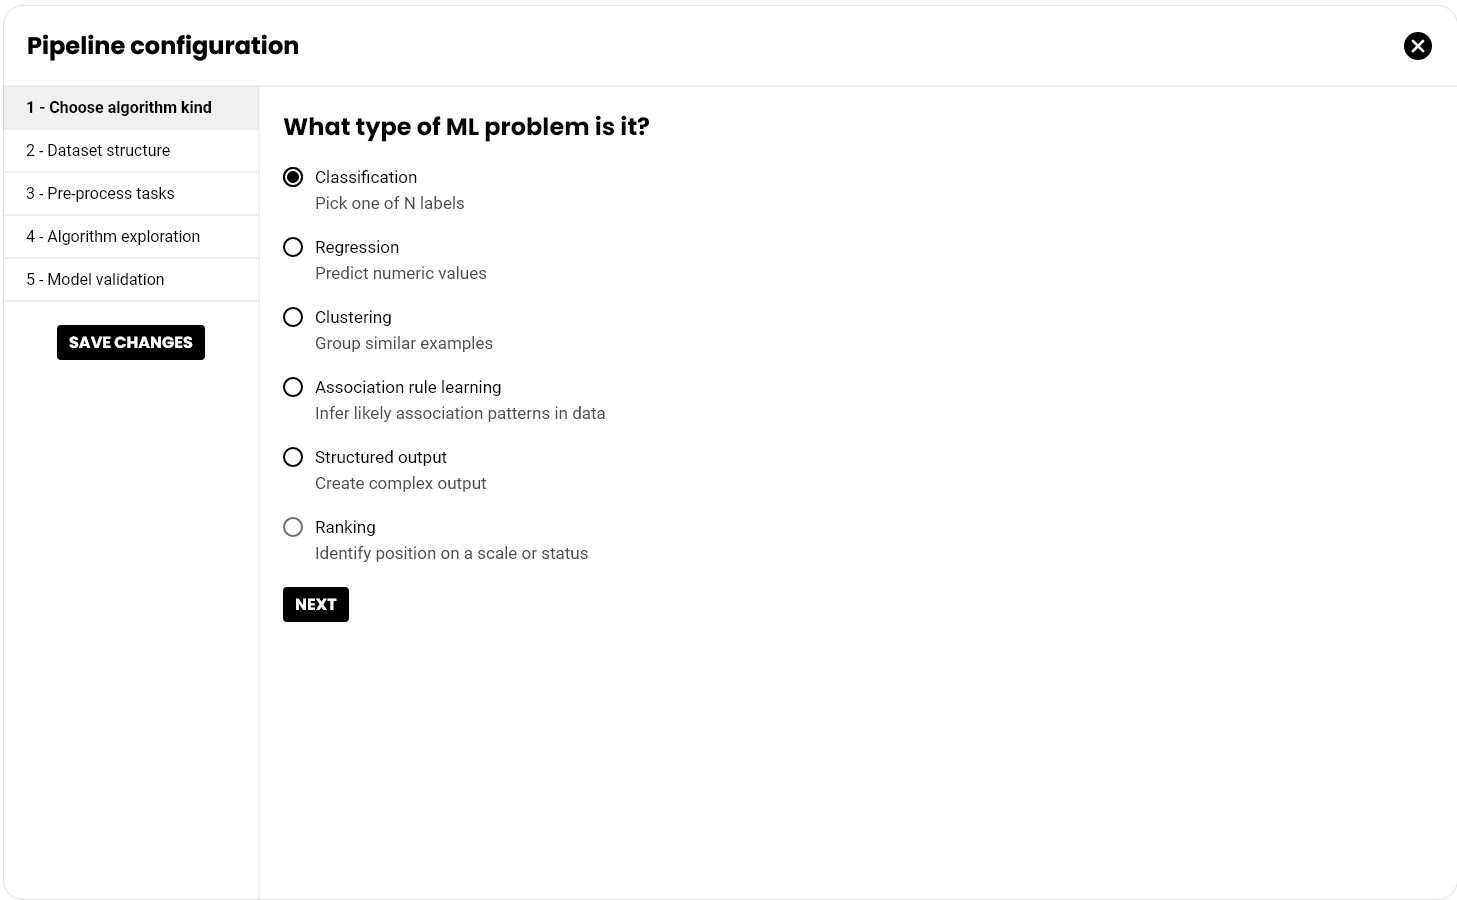
\includegraphics[width=1\textwidth]{chapter-7/advice-steps-config.png}
  \caption{Mock up van een verbeterd configuratie dialoog.}
  \label{fig:ch7-advice-steps-config}
\end{figure}

In de éérste stap in \autoref{fig:ch7-advice-steps-config} is te zien dat de type van het ML probleem wordt gevraagd. Op deze wijze hoeft de developer niet zelf opzoek naar een geschikt algoritme maar kiest welk type ML probleem het is. Op basis hiervan kan de PoC een aantal algoritmes dat het probleem oplost selecteren. Bij stap 5 in \autoref{fig:ch7-advice-steps-config} kan gespecificeerd worden wanneer een model goed genoeg is om uit te rollen. Over het algemeen probeert de PoC relevante opties te geven zodat de developer niet zelf hoeft te programmeren maar simpelweg kan kiezen wat er moet gebeuren.